\documentclass[t,compress,mathserif,10pt,xcolor=dvipsnames, table, aspectratio=43]{beamer}

\usepackage[T1]{fontenc}
\usepackage[utf8]{inputenc}
\usepackage[frenchb]{babel}
\usepackage{eulervm}
\usepackage{etoolbox,refcount}

\usepackage[normalem]{ulem} %strikeout with \sout{}

%%%%% Colors
\definecolor{bleuUni}{RGB}{0, 157, 224}
\definecolor{marronUni}{RGB}{68, 58, 49}
\usecolortheme[named=bleuUni]{structure}
\input{colors}
%%%%%%%%%%%%%%%%%%%

%%%%% Tabs
\usepackage{booktabs}
\usepackage{multirow}
\usepackage{multicol}
\usepackage{makecell}
%\usepackage{enumitem}
%%%%%%%%%%%%%%%%%%%%


%%%%% Plots
\usepackage{pgfplots}
 \pgfplotsset{compat=newest}
 \usepgfplotslibrary{groupplots}
\usepackage{tikz}
  \usetikzlibrary{matrix, positioning, patterns, shapes, arrows, shapes.multipart, decorations.pathmorphing}
\usepackage{circuitikz}
\usepackage{tikz-timing}      % package pour les chronogrammes
\usepackage{caption}
\usepackage{graphicx}
\usepackage[export]{adjustbox} %align in includegraphics
\tikzset{
    invisible/.style={opacity=0},
    visible on/.style={alt={#1{}{invisible}}},
    alt/.code args={<#1>#2#3}{%
      \alt<#1>{\pgfkeysalso{#2}}{\pgfkeysalso{#3}} % \pgfkeysalso doesn't change the path
    },  
}

%%%%%%%%%%%%%%%%%%%%


%%%%% Algo
\usepackage[french,onelanguage, ruled, linesnumbered, vlined]{algorithm2e}
\SetAlFnt{\footnotesize}
%%%%%%%%%%%%%%%%%%%%


%%%%% Math
\usepackage{stmaryrd} %llbracket
\usepackage{amsmath}
\usepackage{amssymb}
\usepackage{marvosym} %grosse fleche
\usepackage{calc}
\DeclareMathOperator{\card}{card}
\DeclareMathOperator*{\maxstar}{max*}
\DeclareMathOperator*{\argmax}{arg\,max}
\DeclareMathOperator*{\decide}{decide}
\DecimalMathComma
%%%%%%%%%%%%%%%%%%%%


%%%%%% Special commands : ddfrac and actionenv and compresslist

\newcommand\ddfrac[2]{\frac{\displaystyle #1}{\displaystyle #2}}

\newenvironment<>{varblock}[2][\textwidth]{%
  \setlength{\textwidth}{#1}
  \begin{actionenv}#3%
    \def\insertblocktitle{#2}%
    \par%
    \usebeamertemplate{block begin}}
  {\par%
    \usebeamertemplate{block end}%
  \end{actionenv}}

\newcommand{\compresslist}{ % Define a command to reduce spacing within itemize/enumerate environments, this is used right after \begin{itemize} or \begin{enumerate}
\setlength{\itemsep}{1pt}
\setlength{\parskip}{0pt}
\setlength{\parsep}{0pt}
}

\newcommand*\circled[1]{\tikz[baseline=(char.base)]{%
      \node[shape=circle,fill=bleuUni,inner sep=2pt] (char) {\textbf{\textcolor{white}{#1}}};}}

\newcommand{\itmsp}[1] {\setlength\itemsep{#1}}
%%%%%%%%%%%%%%%%%%%%%%%%%


%%%%% Beamer
\usepackage[bars]{beamerthemetree} % Beamer theme v 2.2
\mode<presentation>
\newcommand*\oldmacro{}%
\let\oldmacro\insertshorttitle%
\renewcommand*\insertshorttitle{%
 \oldmacro\hfill%
\insertframenumber\,/\,\inserttotalframenumber}
\setbeamertemplate{footline}[frame number]
\setbeamersize{text margin left=10pt,text margin right=10pt}
\setbeamerfont{frametitle}{size=\small}
\setbeamertemplate{frametitle}{ \nointerlineskip %
\begin{beamercolorbox}[wd=\paperwidth,ht=2.2ex,dp=.9ex,left]{frametitle} %
                       \hspace*{2ex}\strut\bfseries\color{bleuUni!15!white}\insertframetitle\strut\par %
\end{beamercolorbox}}

%\setbeamerfont{headline}{size=\footnotesize}

% \usepackage{animate}
% \usepackage{multimedia}
\usetheme{Ilmenau} % Beamer theme v 3.0
\setbeamercolor{section in head/foot}{bg=marronUni}
\useinnertheme{circles} %rectangle bullet points instead of circle ones
\usepackage{beamerthemebars}
\beamertemplatenavigationsymbolsempty
%\setbeamercolor{navigation symbols dimmed}{fg=red!80!black}
%\setbeamercolor{navigation symbols}{fg=red!80!black}
%%%%%%%%%%%%%%%%%%%%%%%%%

\setbeamertemplate{headline}{%
\begin{beamercolorbox}[colsep=1.5pt]{upper separation line head}
\end{beamercolorbox}
\begin{beamercolorbox}{section in head/foot}
    \vskip2pt\insertsectionnavigationhorizontal{\paperwidth}{}{}\vskip2pt
\end{beamercolorbox}%
\begin{beamercolorbox}[ht=10pt]{subsection in head/foot}%
    \vskip2pt\insertsubsectionnavigationhorizontal{\paperwidth}{}{}\vskip2pt
\end{beamercolorbox}%
\begin{beamercolorbox}[colsep=1.5pt]{lower separation line head}
\end{beamercolorbox}
}

\setbeamertemplate{blocks}[rounded][shadow=false]



%%%%% Title
\title{\textbf{Contribution à l'amélioration des \\%
               performances de décodage des turbo codes : \\%
               algorithmes et architecture}}
%\subtitle{algorithms et arhitecture}\hspace{10.7cm}
\author[Thibaud Tonnellier\hspace{7.51cm}{thibaud.tonnellier@ims-bordeaux.fr}]    {Thibaud Tonnellier}
\titlegraphic{
\includegraphics[height=.7cm]{logos/ims.png} \hfil %
              
\includegraphics[height=.7cm]{logos/inp.PNG} \hfil %
              
\includegraphics[height=.7cm]{logos/ub.png}  \hfil %
              
\includegraphics[height=.7cm]{logos/tas.png}}
\date{5 Juillet 2017}
%\pgfdeclareimage[height=.8cm]{le-logo}{logo.png}
%\logo{\pgfuseimage{le-logo}\hspace{\dimexpr\paperwidth-1.55cm}\vspace{-8pt}}
%%%%%%%%%%%%%%%%%%%%%%%%%


%%%%% Contents each new sec and subsec
\AtBeginSection[]
{
  %\ifnumcomp{\value{section}}{=}{1}{}{
    \begin{frame}[c]{Plan}
      \centering
      \tableofcontents[
          currentsection,
          hideothersubsections
          %subsectionstyle=show/hide
      ]
    \end{frame}
  %}
}

\AtBeginSubsection[]
{
  \begin{frame}[c]{Plan}
    \tableofcontents[
      currentsection,
      sectionstyle=show/shaded,
      subsectionstyle=show/shaded/hide
    ]
  \end{frame}
}

%%%%%%%%%%%%%%%%%%%%%%%%%%%%%%%%%%%%%%%%%%%%%%%%%%%%%%%%%%%%%%%%%%%%%%%%%%%%%%%%
\begin{document}

\begin{frame}[c]
  \titlepage
\end{frame}

%%%%%%%%%%%%%%%%%%%%%%%%%%%%%%%%%%%%%%%%%%%%%%%%%%%%%%%%%%%%%%%%%%%%%%%%%%%%%%%%
%\section[]{Contexte}
{
  \usebackgroundtemplate{  \tikz[overlay,remember picture] 
  \node[opacity=0.4, at=(current page.center), inner sep=0pt] {
    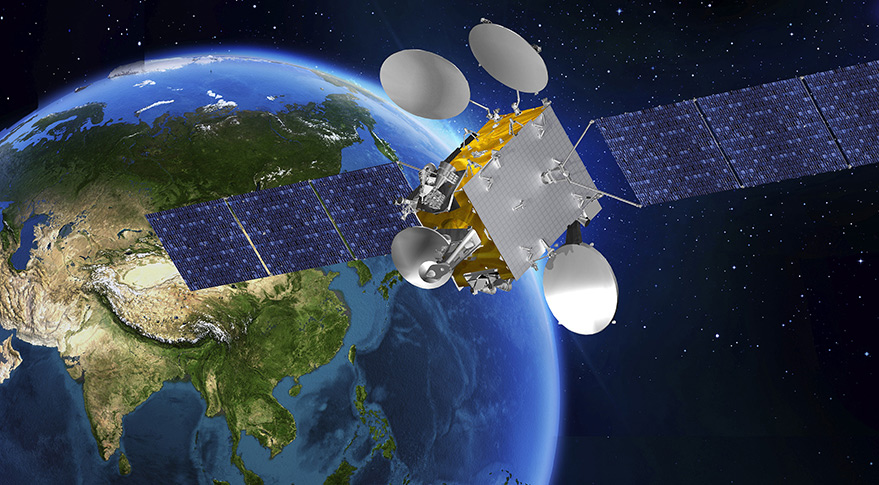
\includegraphics[width=1.2\paperwidth]{fig/sat.jpg}};}
%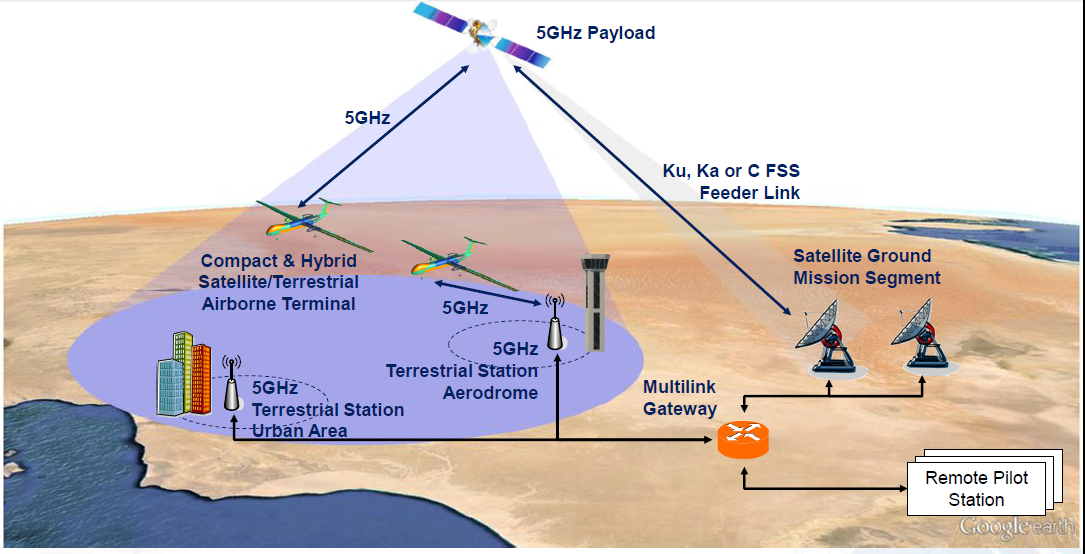
\includegraphics[width=\paperwidth, bottom]{fig/image001.png}}%
\begin{frame}[b]
  \begin{block}{Problématique industrielle}
  	$\color{bleuUni}\bullet$ Un des cœurs de métier de TAS : satellites de télécommunications \\
    $\color{bleuUni}\bullet$ Un standard de communication fige un protocole pour la transmission de l'information\\
    $\color{bleuUni}\bullet$ Or, les besoins applicatifs peuvent évoluer et ne plus correspondre à ceux définis\\
    $\color{bleuUni}\bullet$ Objectif : Améliorer les performances de transmission sans modifier le standard
 \end{block}
\end{frame}
}
\begin{frame}[c]
  \tableofcontents[ 
      subsectionstyle=hide,
  ]
\end{frame}

%%%%%%%%%%%%%%%%%%%%%%%%%%%%%%%%%%%%%%%%%%%%%%%%%%%%%%%%%%%%%%%%%%%%%%%%%%%%%%%%
\section[Introduction]{Introduction et problématique} 

%%%%%%%%%%%%%%%%%%%%%%%%%%%%%%%%%%%%%%%%
\subsection[Le codage de canal]{De la communication au codage de canal}
\begin{frame}{Chaîne de communications numériques simplifiée} 
    \only<1-2>{\includegraphics[width=0.9\textwidth, center,page=2]{fig/shParadigm2.pdf}}
    \only<3>{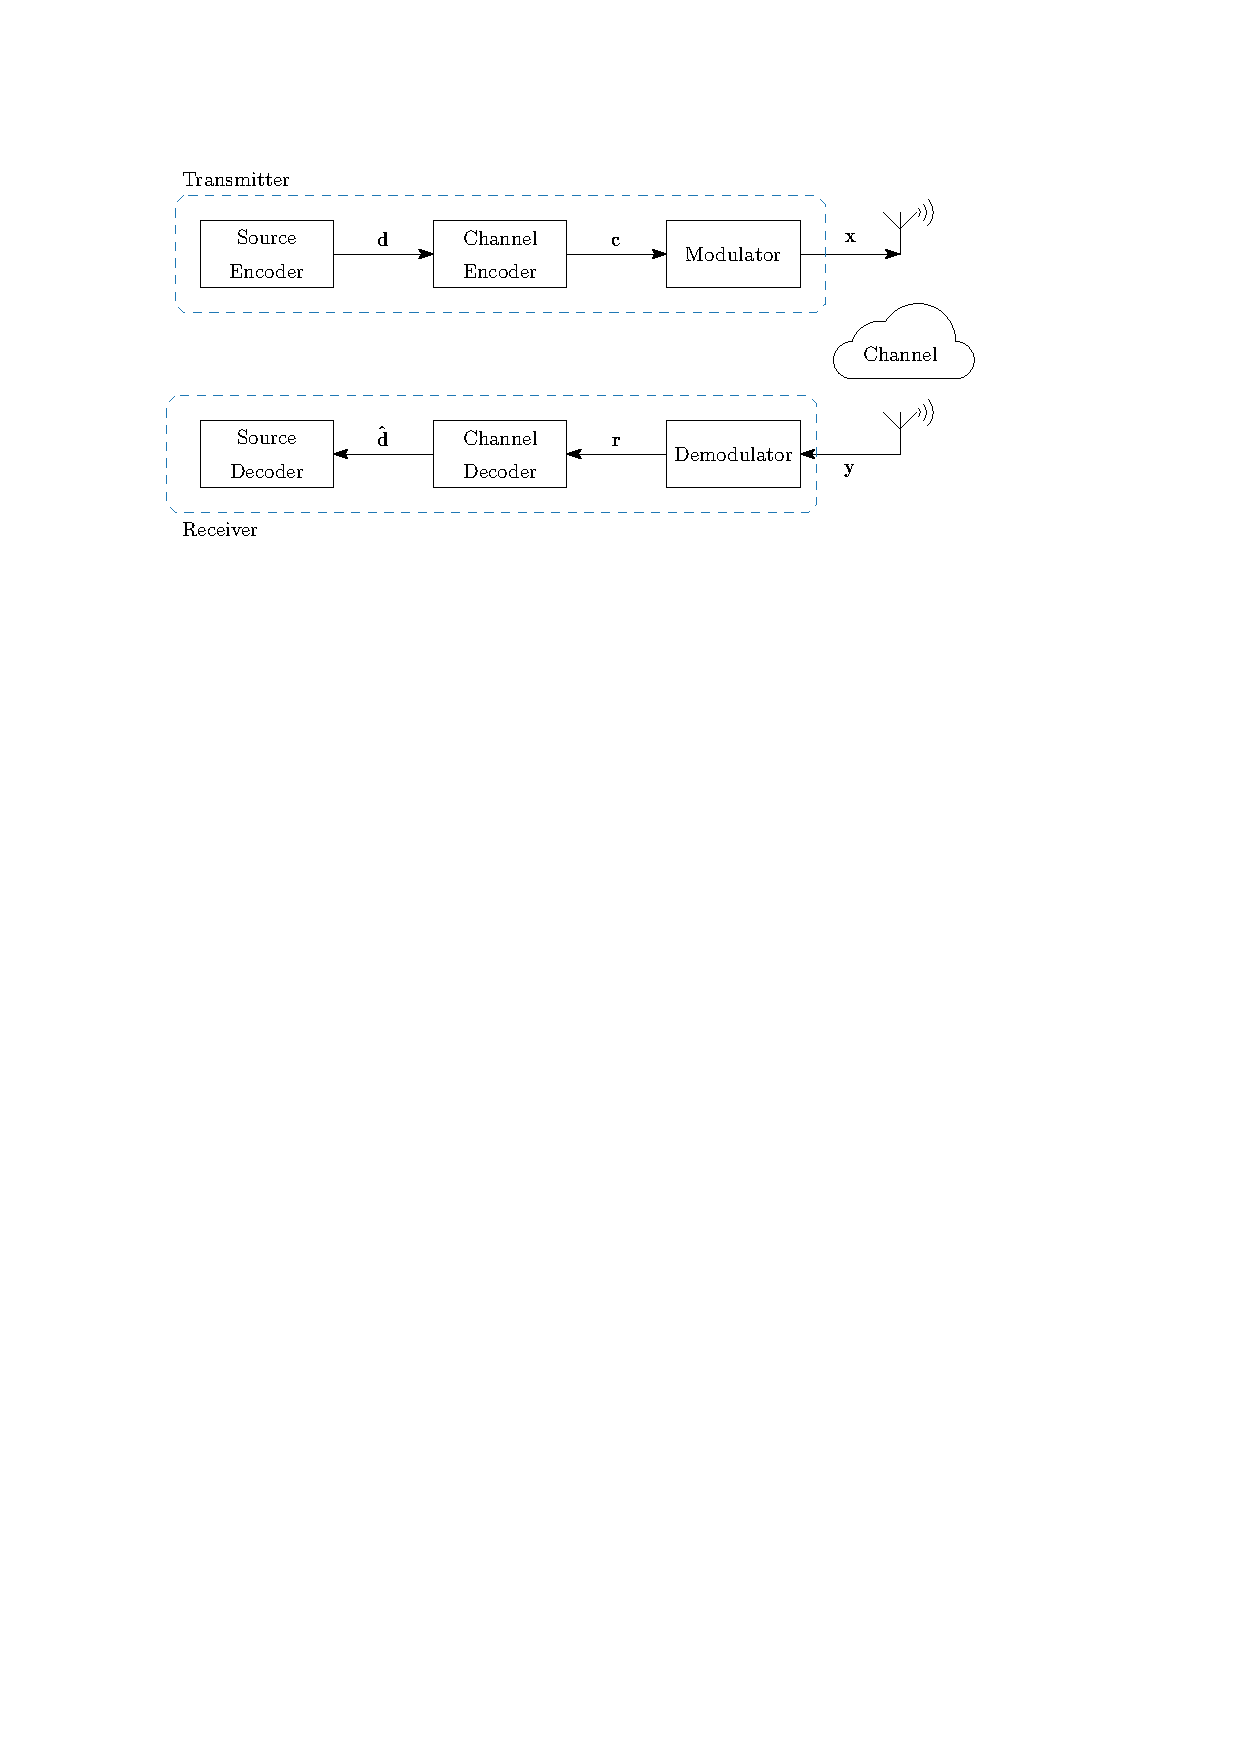
\includegraphics[width=0.9\textwidth, center,page=1]{fig/shParadigm2.pdf}}
   % \only<3>{\includegraphics[width=0.9\textwidth, center,page=3]{fig/shParadigm2.pdf}}
    \only<4>{\includegraphics[width=0.9\textwidth, center,page=4]{fig/shParadigm2.pdf}}
    \only<5>{\includegraphics[width=0.9\textwidth, center,page=5]{fig/shParadigm2.pdf}}
    \only<6>{\includegraphics[width=0.9\textwidth, center,page=6]{fig/shParadigm2.pdf}}
    \vspace*{1ex}
    \only<2-3>{\begin{itemize}\itmsp{.5em}
      \item<2-3> Canal : perturbations (ex : bruit, interférences...)
      \item<3-3> Codage de source : obtenir le maximum de concision dans l’expression d'un message
      \item<3-3> Codage de canal : rendre robuste un message face aux perturbations du canal
    \end{itemize}}
    \only<4-6>{\begin{itemize}\itmsp{.5em}
      \item BPSK : modulation de phase à deux valeurs
      \item AWGN : bruit additif blanc Gaussien\\\vspace*{.5em}
      {\color{bleuUni}\Large\MVRightarrow} les plus utilisés dans la littérature
    \end{itemize}}
\end{frame}

\begin{frame}[t]{Courbes de performances et limites}
\begin{center}
\begin{tikzpicture}
  \begin{semilogyaxis}[footnotesize, width=\linewidth, height=.6\linewidth,    
      %xmin=-1, xmax=10, xtick={-1, 0,...,10},
      xmin=-1, xmax=9, xtick={-1, 0,...,9},
      ymin=1e-5,  ymax=0.15,
      xlabel=$E_b/N_0~\text{(dB)}$, 
      %ylabel=\only<1>{Taux d'erreur binaire}\only<2->{Probabilité et taux d'erreurs binaires},
      ylabel=Taux d'erreur binaire,
      grid=both, grid style={gray!30},
      tick align=outside, tickpos=left, % legend columns=2, legend style={at={(1, -.25), anchor=north}, /tikz/column 2/.style={column sep=5pt}} 
      ]

      \addplot[mark=none,Paired-5, semithick, visible on=<2->]  table [x=SNR, y=BER] {../main/ch1_fig/berBPSK.dat}; \label{bpsk}

      %\addplot[<->, visible on=<4->]                            coordinates          {(5.4, 1e-4   ) (8.3, 1e-4)}; 
      %\addplot[<->, visible on=<5->]                            coordinates          {(5  , 2.05e-4) (5  , 6e-3)};
      \addplot[mark=none, Paired-3, thick, visible on=<3->] coordinates {(0.187,0.000001)(0.187,0.2)};              \label{shann}
      \addplot[mark=o,   Paired-1, semithick, visible on=<5->]  table [x=SNR, y=BER] {../main/ch1_fig/berRSC.dat};  \label{rsc}
      \addplot[mark=triangle,   Paired-7, semithick, visible on=<8->, restrict x to domain=0:0.7]  table [x=SNR, y=BER2] {data/berrou.txt}; \label{tc}
      \draw[pattern=north west lines, draw=none, pattern color=Paired-7, visible on=<4->] (axis cs:-1,1e-6) rectangle (axis cs:0.184, 1e-3);%
                %\addlegendimage{pattern=north west lines, draw=none, pattern color=Paired-7,  area legend};
      \addplot [<->, visible on=<6->] coordinates {(5.4, 1e-4) (8.3, 1e-4)};
      \addplot [<->, visible on=<7->] coordinates {(5, 2e-4) (5, 5e-3)};
      

      \coordinate (legend) at (axis description cs:.9, -.21);
      \legend{Non codé, Limite de Shannon R=1/2, Code convolutif R=1/2, Turbo code R=1/2}
  \end{semilogyaxis}
    % \only<2>{\matrix [matrix of nodes, anchor=north east, fill=white,  ampersand replacement=\&] at (legend) 
    %          {\ref{bpsk} \& \qquad \footnotesize{Non codé}\qquad\qquad  \&  \qquad~~ \& \qquad  \qquad \qquad  \qquad \\
    %          \qquad \& \qquad\qquad \& \qquad \& \qquad\qquad \\ };}
    % \only<3-5>{\matrix [ matrix of nodes, anchor=north east, fill=white,  ampersand replacement=\&] at (legend) 
    %          {\ref{bpsk} \& \qquad  \footnotesize{~~~~Non codé~~~~} \qquad\qquad \& \ref{rsc} \& \footnotesize{Code RSC R=1/2~} \\
    %          \qquad \& \qquad\qquad \& \qquad \& \qquad\qquad \\};}             
    % \only<6-7>{\matrix [ matrix of nodes, anchor=north east, fill=white,  ampersand replacement=\&] at (legend) 
    %          {\ref{bpsk} \& \footnotesize{Non codé} \& \ref{rsc} \& \footnotesize{Code RSC R=1/2~} \\
    %          \ref{shann} \& \footnotesize{Limite de Shannon R=1/2}  \\};}  
    %  \only<8>{\matrix [ matrix of nodes, anchor=north east, fill=white,  ampersand replacement=\&] at (legend) 
    %          {\ref{bpsk} \& \footnotesize{Non codé} \& \ref{rsc} \& \footnotesize{Code RSC R=1/2~} \\
    %          \ref{shann} \& \footnotesize{Limite de Shannon R=1/2}  \& \ref{tc} \& \footnotesize{Turbo code R=1/2}\\};}   
\end{tikzpicture}  
\end{center}
\end{frame} 

%%%%%%%%%%%%%%%%%%%%%%%%%%%%%%%%%%%%%%%%
\subsection{Les turbo codes}
\begin{frame}[c]{Vue d'ensemble}
  \begin{center}
    \only<1> {\includegraphics[width=.8\textwidth, page=4]{fig/shParadigm2.pdf}}
    \only<2->{\includegraphics[width=.8\textwidth, page=7]{fig/shParadigm2.pdf}}
  \end{center}
  \vspace*{-1em}
  \begin{itemize}\itmsp{.5em}
    \item<2-> L'un des codes correcteur d'erreurs les plus efficaces
    \item<3> Excellent compromis entre la complexité calculatoire et les performances de décodage
        \item<3> Choisis dans plusieurs standards de communication numérique sans-fil :
          \begin{itemize}
            \item Contexte satellitaire (CCSDS, DVB-RCS)
            \item Contexte mobile (LTE)
          \end{itemize}
  \end{itemize}
\end{frame}

\begin{frame}[c]{Turbo codeur}
  \begin{center}
    \only<1>{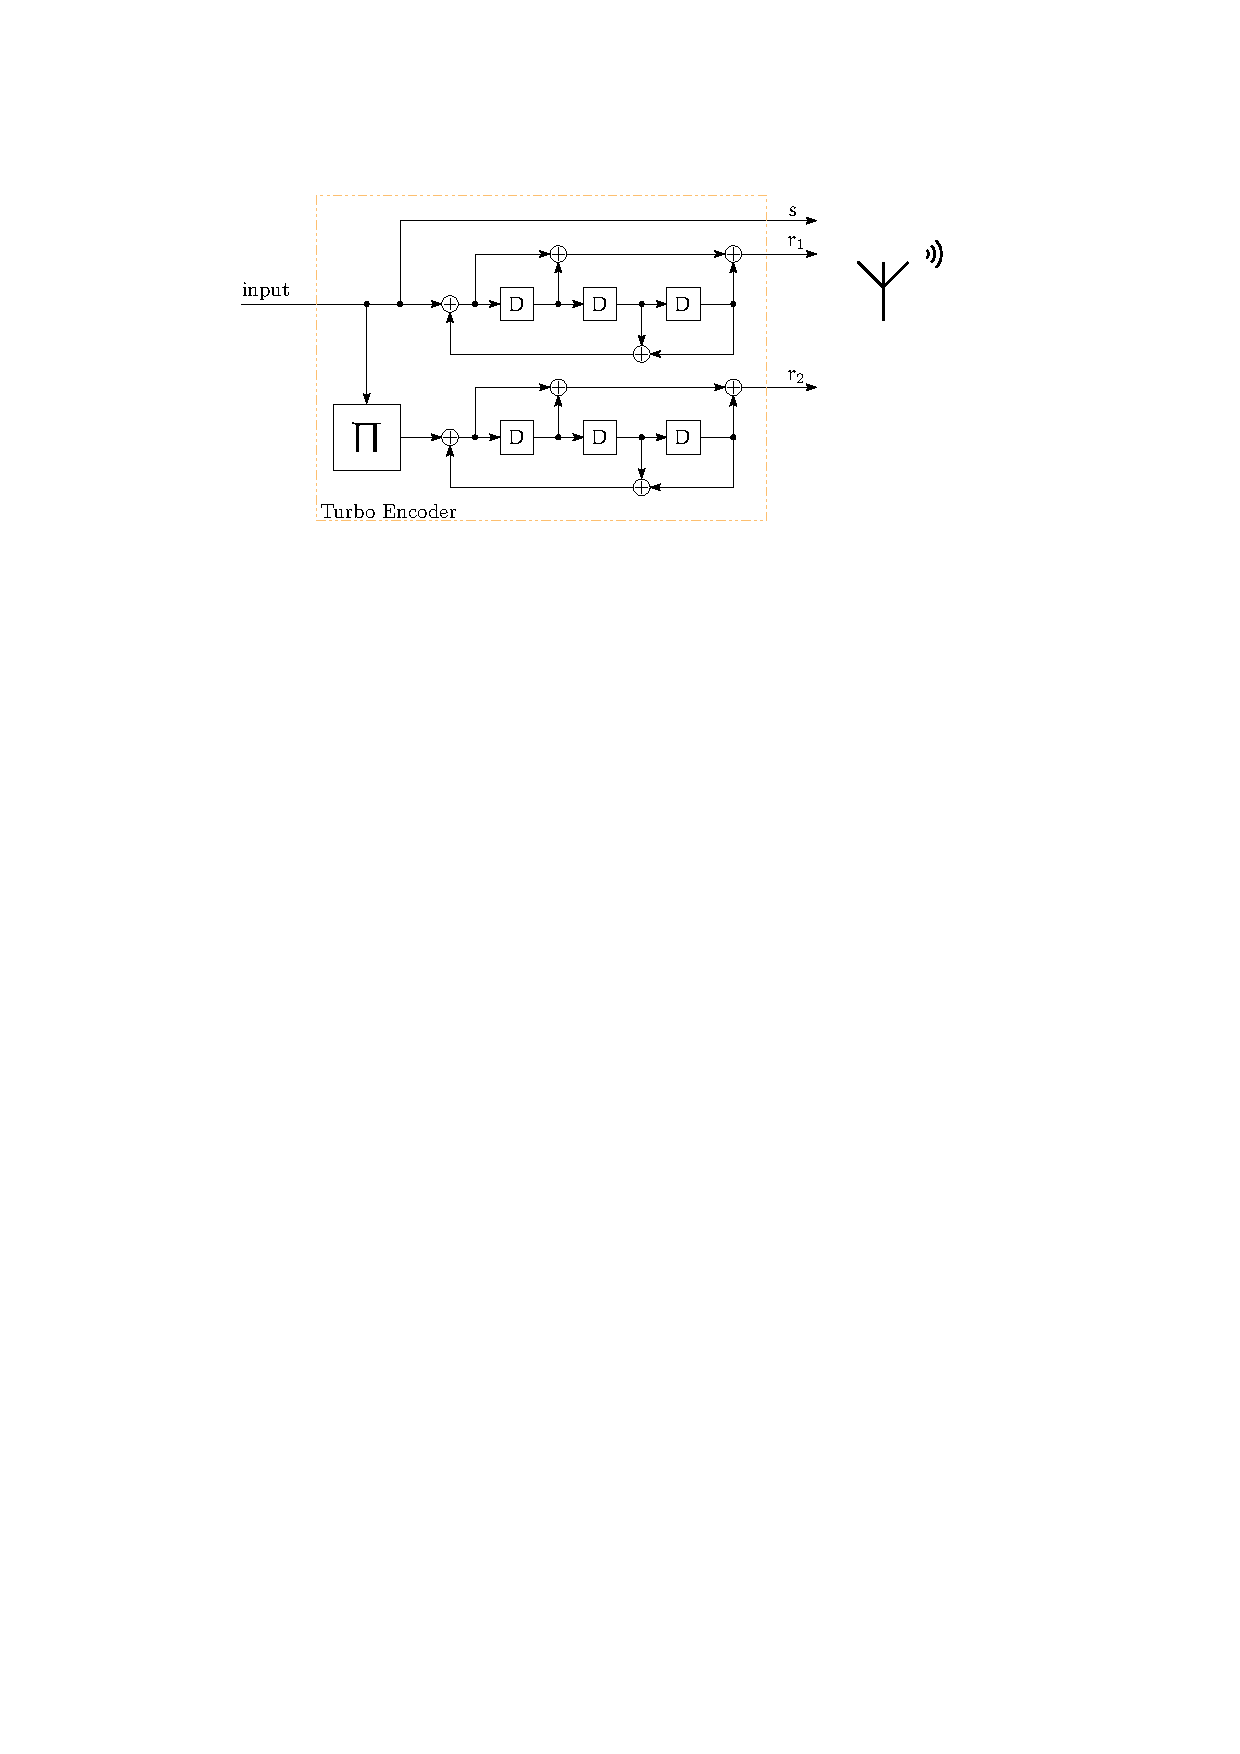
\includegraphics[width=.9\textwidth,page=1]{fig/encoder.pdf}}
    \only<2>{\includegraphics[width=.9\textwidth,page=2]{fig/encoder.pdf}}
    \only<3>{\includegraphics[width=.9\textwidth,page=3]{fig/encoder.pdf}}
  \end{center} 
  \begin{itemize}\itmsp{.5em}
    \item Trois blocs élémentaires : 2 codeurs convolutifs + entrelaceur ($\Pi$)
    \item Rendement natif : 1/3 $\mathbf{c = [s,~p_1,~p_2]}$ \only<3>{\qquad $\color{bleuUni}\bullet$ Représentation en treillis}
  \end{itemize}
\end{frame} 
 
\begin{frame}[fragile]{Turbo décodeur}
\begin{overlayarea}{\textwidth}{\textheight}
    \only<1>{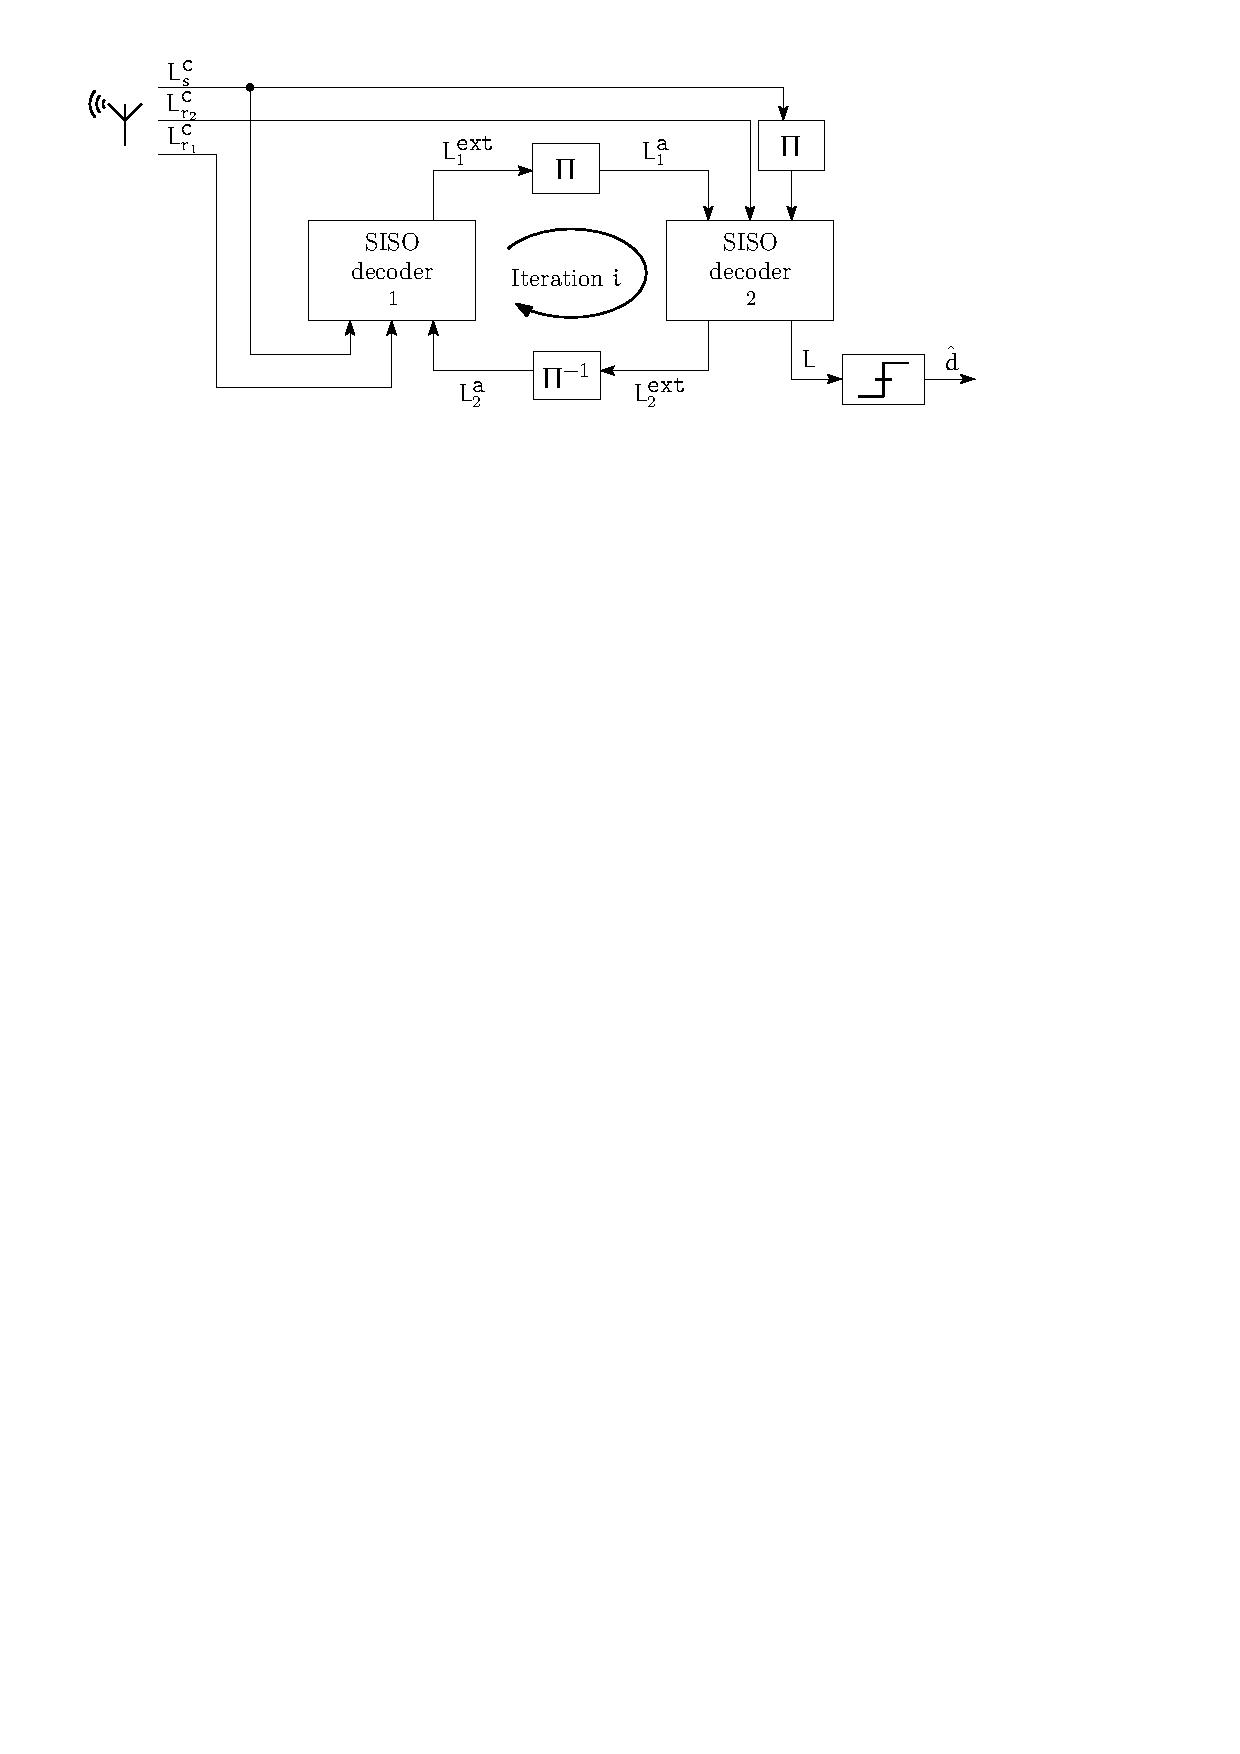
\includegraphics[width=\textwidth,page=1, center]{fig/tdec.pdf}}
    \only<2>{\includegraphics[width=\textwidth,page=2, center]{fig/tdec.pdf}}
    \only<3>{\includegraphics[width=\textwidth,page=3, center]{fig/tdec.pdf}}
    \only<4>{\includegraphics[width=\textwidth,page=4, center]{fig/tdec.pdf}}
    \only<5>{\includegraphics[width=\textwidth,page=3, center]{fig/tdec.pdf}}
    \only<6>{\includegraphics[width=\textwidth,page=5, center]{fig/tdec.pdf}}
    \only<1-5>{\vspace*{-2.5em}}
    \only<6>{\vspace*{-2.5em}}

    \only<1->{$\color{bleuUni}\bullet$ Composé de 2 SISOs et d'entrelaceurs/désentrelaceurs \\}
    \only<2->{$\color{bleuUni}\bullet$ Processus itératif : SISOs échangent leurs avis via l'information extrinsèque ($\mathbf{L^{e}}$)}
\end{overlayarea}
\end{frame}


\begin{frame}[c]{Performances - LTE - K = 2048 - R=1/3 - 8 its - Flottant - AWGN - BPSK}
\begin{columns}[T] % align columns
\begin{column}{.5\textwidth}
\begin{center}
\vspace*{-1.5em}
  \begin{tikzpicture}
  \begin{semilogyaxis}[footnotesize, width=\linewidth, height=1.3\linewidth,
      xmin=0, xmax=2.2, xtick={0,0.4,...,2.2},
      ymin=2e-7,  ymax=1.1,
      xlabel=$E_b/N_0 \text{(dB)}$, ylabel=FER,  grid=both, grid style={gray!30},
     tick align=outside, tickpos=left, legend pos=north east]
                                                                       
      \addplot[mark=o,Paired-5]  table [x=SNR, y=FER] {../main/ch1_fig/std/lte13_2048.dat};                            
      %\addplot[Paired-6]  table [x=SNR, y=FER] {../main/ch1_fig/std/lte13_2048_ubound.dat};
      % \addplot [draw=none,fill=red!20, semitransparent, visible on=<2->] coordinates {(-1,1e-7) (-1,1) (0.3,1) (0.3,1e-7)};
      % \addplot [draw=none,fill=green!20, semitransparent, visible on=<3->] coordinates {(0.3,1e-7) (0.3,1) (1.0,1) (1.0,1e-7)};
      % \addplot [draw=none,fill=blue!20, semitransparent, visible on=<4->] coordinates {(1.0,1e-7) (1.0,1) (2.0,1) (2.0,1e-7)};
      \addplot [draw=none,fill=Paired-1!50, semitransparent, visible on=<2->] coordinates {(0,2e-1) (0,2) (0.4,2) (0.4,0.1)};
      \addplot [draw=none,fill=Paired-3!50, semitransparent, visible on=<3->] coordinates {(0.4,0.1) (0.4,2) (1.1,4e-5) (1, 6e-6)};
      \addplot [draw=none,fill=Paired-7!50, semitransparent, visible on=<4->] coordinates {(1,6e-6) (1.1,4e-5) (1.7,3e-6) (1.7,7e-7)};
      %\addplot [draw=green,fill=blue, semitransparent] coordinates {(-360,-1.1) (-360,1.1) (55,1.1) (55,-1.1)};
      % \only<2->{\draw[rotate=70] (0.0,0.9) ellipse (0.25cm and .8cm);}
      % \only<3->{\draw[rotate=15] (0.4,0.001) ellipse (0.25cm and 1.8cm);}
      % \only<4->{\draw[rotate=70] (0.3,1) ellipse (0.25cm and 1cm);}
      \legend{TC}
                                                                                                
  \end{semilogyaxis}
\end{tikzpicture}
%\captionof{figure}{\small Standard LTE, R=1/3, K=2048, Canal AWGN, 8 itérations EML-MAP, borne de l'union}
\end{center}
\end{column}%
\hfill%
\begin{column}{.5\textwidth}
% \vspace*{2em}
% \visible<2->{$\color{bleuUni}\bullet$ Manifestation :\\
% La courbe de performances s’aplatit à fort SNR}

% % \vspace*{1em}
% % \visible<3->{$\color{bleuUni}\bullet$ Cause : \\
% % Distribution des mots de code possédant un faible poids ($d_\text{min}$)}

% % \vspace*{1em}
% % \visible<4->{$\color{bleuUni}\bullet$ Propriété : \\
% % Erreurs résiduelles en sont responsables (faible BE/FE)}
% \vspace*{3em}
% \visible<3->{$\color{bleuUni}\bullet$ Problème : \\
% Empêche l'obtention de très faible taux d'erreurs pour de faibles SNR.}
\begin{itemize}\itmsp{1em}
  \item Cette courbe de performance = Cas d'étude
  \item Trois zones :
  \begin{itemize}\itmsp{2em}
    \item <2-> Non convergence
    \item <3-> Convergence (waterfall)
    \item <4-> Plancher d'erreurs (error floor)
    \begin{itemize}
      \item <4-> La courbe de performances s’aplatit à fort SNR
      \vspace*{1em}
      \item <4-> Empêche l'obtention de très faible taux d'erreurs pour de faibles SNR.
    \end{itemize}
  \end{itemize}
\end{itemize}
\end{column}%
\end{columns}
\end{frame}

\begin{frame}{Quelles solutions ?}
\begin{enumerate}
  \item \only<2->{\sout}{Modifier le code}
  \begin{itemize}
    \item<1> Entrelaceur
    \item<1> Nombre d'états du codeur
    \item<1> Concaténation (BCH, RSC-1 par exemple)
  \end{itemize}
  \item<3-> Modifier l'algorithme de décodage
  \begin{itemize}
    \item<4-> Modifier l'échange de l'information extrinsèque 
    \begin{itemize}
      \item<5-> Facteur de remise à l'échelle (scaling factor) [1]
    \end{itemize}
    \item<6-> Exploiter un code détecteur d'erreurs (CRC) présent dans la majorité des standards
    \begin{itemize}
      \item<7-> Décodage par liste [2]
      \item<7-> Décodage par statistiques ordonnées [3]
      \item<7-> Décodages successifs d'une même trame [4]
    \end{itemize}
    \vspace*{.5em}
    \item<8-> Propositions :
    \begin{itemize}
      \item<9-> Self-Corrected [Chapitre II du manuscrit]
      \item<10-> Flip and Check (FNC) [Chapitre III du manuscrit]\\
    \end{itemize}
  \end{itemize}
\end{enumerate}
\vspace*{1ex}
\only<5->{\let\thefootnote\relax\footnotetext{\tiny [1] Vogt et al.,"Improving the Max-Log-MAP turbo decoder", Electron. Lett., 2000}}
\only<7->{\let\thefootnote\relax\footnotetext{\tiny [2] Akmalkhodzhaev et al.,"New iterative turbo code list decoder", REDUNDANCY, 2014}}
\only<7->{\let\thefootnote\relax\footnotetext{\tiny [3] Xu et al.,"An efficient {OSD}-aided iterative decoding algorithm for {LTE} turbo codes", WCSP, 2012}}
\only<7->{\let\thefootnote\relax\footnotetext{\tiny [4] Crozier et al.,"Improving the Error Rate Performance of Turbo Codes using the Forced Symbol Method", Commun. Lett., 2007}}
\end{frame}

%%%%%%%%%%%%%%%%%%%%%%%%%%%%%%%%%%%%%%%%%%%%%%%%%%%%%%%%%%%%%%%%%%%%%%%%%%%%%%%%
\section[Erreurs résiduelles]{Erreurs résiduelles : identification et correction}
%%%%%%%%%%%%%%%%%%%%%%%%%%%%%%%%%%%%%%%%
\subsection{Observations dans la zone du plancher d'erreurs}

\begin{frame}[c]{Exemple standard LTE, K=2048, R=1/3 - Nombre moyen de bits erronés par trame}
\begin{columns}[T] % align columns
  \begin{column}{.5\textwidth}
    %\begin{center}
    \begin{tikzpicture}
      \begin{semilogyaxis}[footnotesize, width=\linewidth, height=1.3\linewidth,
                          xmin=0, xmax=2.2, xtick={0,0.4,...,2.2},
                          %ymin=2e-6,  ymax=0.11,
                          xlabel=$E_b/N_0 \text{(dB)}$, ylabel=FER,  grid=both, grid style={gray!30},
                          tick align=outside, tickpos=left, legend pos=north east]
                                                                     
        \addplot[mark=o,Paired-5]  table [x=SNR, y=FER] {../main/ch1_fig/std/lte13_2048.dat}; 
         \addplot [draw=none,fill=Paired-7!50, semitransparent, visible on=<3->] coordinates {(1,6e-6) (1.1,2e-5) (1.7,3e-6) (1.7,7e-7)};                           
                                                                                                       
        \legend{TC}                                                                                        
      \end{semilogyaxis}
    \end{tikzpicture}
    %\end{center}
  \end{column}%
  \hfill%
  \begin{column}{.5\textwidth}
  %\begin{center}
 % \vspace{-1ex}
    \begin{tikzpicture}
      \begin{axis}[footnotesize, width=\linewidth, height=1.3\linewidth,
                   xmin=0, xmax=2.2, xtick={0,0.4,...,2.2},
                   ymin=0,  ymax=295,
                    xlabel=$E_b/N_0 \text{(dB)}$, ylabel=BE/FE,  grid=both, grid style={gray!30},
                    tick align=outside, tickpos=left, legend pos=north east]
                                                                       
          \addplot[mark=o,Paired-5, visible on=<2->]  coordinates  {(0.0, 286)  (0.1, 218)  (0.2, 199) (0.3, 112) (0.4, 92) (0.5, 79) (0.6, 77) (0.7, 59) (0.8, 57) 
                                                                   (0.9, 42.6) (1.0, 16.3) (1.1, 4.4) (1.2, 4.0) (1.3, 3.5) (1.4, 4.8) (1.5, 3.3)(1.6, 3.2)};
        \addplot [draw=none,fill=Paired-7!50, semitransparent, visible on=<3->] coordinates {(1.05,0) (1.05,10) (1.7,10) (1.7,0)};                           
                                                                                                         
          \legend{TC}                                                                                        
      \end{axis}
    \end{tikzpicture}
    %\end{center}
  \end{column}%
\end{columns}
\end{frame}


\begin{frame}[c]{Exemple standard LTE, K=2048, R=1/3 - Distribution des erreurs binaires}
\begin{columns}[T] % align columns
  \begin{column}{.3\textwidth}
      \begin{tikzpicture}
      \begin{semilogyaxis}[footnotesize, width=1.1\linewidth, height=2\linewidth,
                          xmin=0, xmax=2.2, xtick={0,0.4,...,2.2},
                          %ymin=2e-6,  ymax=0.11,
                          xlabel=$E_b/N_0 \text{(dB)}$, ylabel=FER,  grid=both, grid style={gray!30},
                          tick align=outside, tickpos=left, legend pos=north east]
                                                                     
        \addplot[mark=o,Paired-5]  table [x=SNR, y=FER] {../main/ch1_fig/std/lte13_2048.dat}; 
         \addplot[mark=*, Paired-1, mark size =2, visible on=<2->]  coordinates {(0.9, 1.23e-04)};                    
         \addplot[mark=*, Paired-3, mark size =2, visible on=<3->]  coordinates {(1.1, 1.00e-05)};                    
         \addplot[mark=*, Paired-5, mark size =2, visible on=<4->]  coordinates {(1.3, 4.31e-06)};                    
                                                                                                       
        \legend{TC}                                                                                        
      \end{semilogyaxis}
    \end{tikzpicture}
  \end{column}%
  \hfill%
  \begin{column}{.7\textwidth}
  \vspace*{2em}
   \begin{tikzpicture}
     \begin{axis}[footnotesize, 
           height=.6\textwidth,  width=\textwidth,
           grid=both, grid style={gray!30},
           %colorbrewer cycle list=Spectral,
           ybar interval=1pt, %/pgf/bar width=3pt,
           xmin=1, xmax=22, xtick={1,2,...,22}, ymin=0,  ytick={0,10,...,45}, ymax=45, 
           grid=both, grid style={dashed, gray!50},  legend style={at={(0.5,1.03)},anchor=south},legend columns=4,
           xticklabels={1,2,3,4,5,6,7,8,9,10,11,12,13,14,15,16,17,18,19,20,>20},
           x tick label style={shift={(axis cs:1.25,0)},anchor=east,rotate=60},
           restrict y to domain*=0:45, % Cut values off at 14
           visualization depends on=rawy\as\rawy, % Save the unclipped values
           after end axis/.code={\draw [ultra thick, white, decoration={snake, amplitude=1pt}, decorate] (rel axis cs:0,0.95) -- (rel axis cs:1,0.95);},
           axis lines*=left,
           clip=false,
           xlabel = Nombre d'erreurs binaires,
           ylabel = Distribution (\%),
           legend style={at={(0.5,1.03)},anchor=south}, legend columns=4,
           ]
   
          \addplot[draw=Paired-1, fill=Paired-1!50, postaction={pattern color = black!80,pattern=north west lines}, visible on=<2->] table [x=X, y expr=\thisrowno{5}/5] {../main/ch3_fig/be/dat/2048.dat};
          \addplot[draw=Paired-3, fill=Paired-3!50, postaction={pattern color = black!80,pattern=north east lines}, visible on=<3->] table [x=X, y expr=\thisrowno{6}/5] {../main/ch3_fig/be/dat/2048.dat};
          \addplot[draw=Paired-5, fill=Paired-5!50, postaction={pattern color = black!80,pattern=crosshatch dots }, visible on=<4->] table [x=X, y expr=\thisrowno{7}/5] {../main/ch3_fig/be/dat/2048.dat};
         % \addplot[mark=*, only marks, black, mark options={scale=0.9, fill=Dark2-2!50 }, update limits=false, visible on=<5->] table[x=X, y=l2048] {../main/ch3_fig/be/dat/th};

          \legend{$0.9$ dB,$1.1$ dB,$1.3$ dB}%, Théorique $1.3$ dB}

          \end{axis}
   \end{tikzpicture}
%\end{center}
  \end{column}%
\end{columns}
\end{frame}

%%%%%%%%%%%%%%%%%%%%%%%%%%%%%%%%%%%%%%%%
\subsection{Identification des positions des bits erronés}
\begin{frame}[c]{Le critère d'identification retenu}
\only<1>{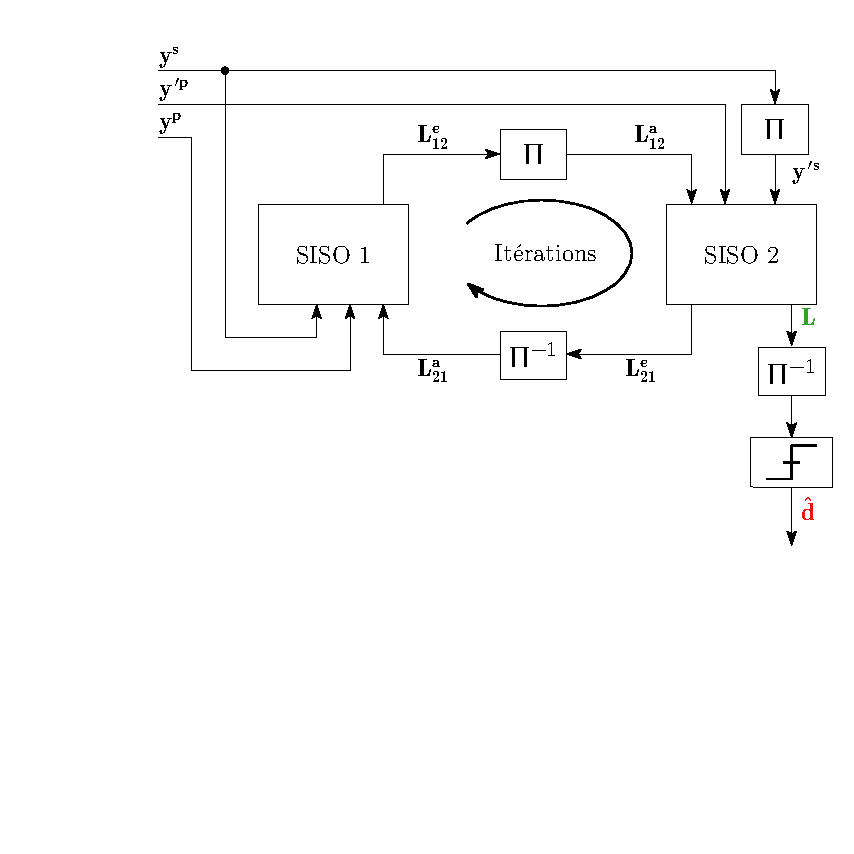
\includegraphics[width=.7\textwidth,page=1, center]{fig/delta.pdf}}
\only<2>{\includegraphics[width=.7\textwidth,page=2, center]{fig/delta.pdf}}
\only<3>{\includegraphics[width=.7\textwidth,page=3, center]{fig/delta.pdf}}
\vspace*{-1.8em}
\begin{itemize}%\setlength\itemsep{.4em}
  \item<3->  $    \Delta(k) = |L(k)|, \qquad \text{avec k~}\in \llbracket0;~K \rrbracket $
  \item<3-> Module de l'information \textit{a posteriori} {\color{bleuUni}\Large\MVRightarrow} niveau de confiance associé à chaque bit du
mot décodé
  \item<3-> Corrélation forte entre une information \textit{a posteriori} faible et une erreur de décodage
\end{itemize}
\end{frame}

\begin{frame}[fragile]{Résultats d'identification -  Standard LTE, K=2048, R=1/3}
\begin{columns}[T] % align columns
  \begin{column}{.48\textwidth}
  \vspace*{4em}
   \begin{tikzpicture}
     \begin{axis}[footnotesize, 
           height=.6\textwidth,  width=\textwidth,
           grid=both, grid style={gray!30},
           %colorbrewer cycle list=Spectral,
           ybar interval=1pt, %/pgf/bar width=3pt,
           xmin=1, xmax=11, xtick={1,2,...,11}, ymin=0,  ytick={0,10,...,45}, ymax=45, 
           grid=both, grid style={dashed, gray!50},  legend style={at={(0.5,1.03)},anchor=south},legend columns=4,
           xticklabels={1,2,3,4,5,6,7,8,9,10},
           x tick label style={shift={(axis cs:1.25,0)},anchor=east,rotate=60},
           restrict y to domain*=0:45, % Cut values off at 14
           visualization depends on=rawy\as\rawy, % Save the unclipped values
           after end axis/.code={\draw [ultra thick, white, decoration={snake, amplitude=1pt}, decorate] (rel axis cs:0,0.95) -- (rel axis cs:1,0.95);},
           axis lines*=left,
           clip=false,
           xlabel = Erreurs binaires,
           ylabel = Distribution (\%),
           legend style={at={(0.5,1.03)},anchor=south}, legend columns=4,
           ]
   
         % \addplot[draw=Paired-1, fill=Paired-1!50, postaction={pattern color = black!80,pattern=north west lines}, visible on=<2-6>, restrict x to domain=1:11] table [x=X, y expr=\thisrowno{5}/5] {../main/ch3_fig/be/dat/2048.dat};
         % \addplot[draw=Paired-3, fill=Paired-3!50, postaction={pattern color = black!80,pattern=north east lines}, visible on=<7-11>, restrict x to domain=1:11] table [x=X, y expr=\thisrowno{6}/5] {../main/ch3_fig/be/dat/2048.dat};
          \addplot[draw=Paired-5, fill=Paired-5!50, postaction={pattern color = black!80,pattern=crosshatch dots }, visible on=<2-6>, restrict x to domain=1:11] table [x=X, y expr=\thisrowno{7}/5] {../main/ch3_fig/be/dat/2048.dat};
          %\addplot[mark=*, only marks, black, mark options={scale=0.9, fill=Dark2-2!50 }, update limits=false, visible on=<5->] table[x=X, y=l2048] {../main/ch3_fig/be/dat/th};

          \legend{$1.3$ dB}%, Théorique $1.3$ dB}

          \end{axis}
   \end{tikzpicture}
  \end{column}%
  \hfill%
  \begin{column}{.48\textwidth}
      \only<1>{
    \begin{tikzpicture}
    \begin{axis}[
    height=.8\textheight,  width=\textwidth, grid=both, grid style={gray!30}, ybar interval = 1pt, /pgf/bar width=-5pt, xmin=1, xmax=6, ymin=0,  ytick={0,10,...,105}, ymax=105, 
          grid=both, grid style={dashed, gray!50},  legend style={at={(0.5,1.05)},anchor=south},legend columns=4, xticklabels={4, 6, 8, 10, 20}, ylabel=Identification réussie (\%),
          x tick label style={shift={(axis cs:1.15,-2.5)},anchor=east}, axis lines*=left, xlabel=Nombre de bits considérés ($q$), legend entries = {Métrique $\Delta$} ]
        \addplot[draw=none] table [x=X, y expr=\thisrowno{2}/5.0, restrict x to domain=0:2] {../main/ch3_fig/id2/dat/2048};
    \end{axis}
   \end{tikzpicture}}
    \only<2>{
    \begin{tikzpicture}
    \begin{axis}[
    height=.8\textheight,  width=\textwidth, grid=both, grid style={gray!30}, ybar interval = 1pt, /pgf/bar width=-5pt, xmin=1, xmax=6, ymin=0,  ytick={0,10,...,105}, ymax=105, 
          grid=both, grid style={dashed, gray!50},  legend style={at={(0.5,1.05)},anchor=south},legend columns=4, xticklabels={4, 6, 8, 10, 20}, ylabel=Identification réussie (\%),
          x tick label style={shift={(axis cs:1.15,-2.5)},anchor=east}, axis lines*=left, xlabel=Nombre de bits considérés ($q$), legend entries = {Métrique $\Delta$} ]
        \addplot[draw=marronUni!50!black, fill=Paired-5!50] table [x=X, y expr=\thisrowno{6}/5.0, restrict x to domain=0:2] {../main/ch3_fig/id2/dat/2048};
    \end{axis}
   \end{tikzpicture}}
    \only<3>{
    \begin{tikzpicture}
    \begin{axis}[
    height=.8\textheight,  width=\textwidth, grid=both, grid style={gray!30}, ybar interval = 1pt, /pgf/bar width=-5pt, xmin=1, xmax=6, ymin=0,  ytick={0,10,...,105}, ymax=105, 
          grid=both, grid style={dashed, gray!50},  legend style={at={(0.5,1.05)},anchor=south},legend columns=4, xticklabels={4, 6, 8, 10, 20}, ylabel=Identification réussie (\%),
          x tick label style={shift={(axis cs:1.15,-2.5)},anchor=east}, axis lines*=left, xlabel=Nombre de bits considérés ($q$), legend entries = {Métrique $\Delta$} ]
        \addplot[draw=marronUni!50!black, fill=Paired-5!50] table [x=X, y expr=\thisrowno{6}/5.0, restrict x to domain=0:3] {../main/ch3_fig/id2/dat/2048};
    \end{axis}
   \end{tikzpicture}}
   \only<4>{
    \begin{tikzpicture}
    \begin{axis}[
    height=.8\textheight,  width=\textwidth, grid=both, grid style={gray!30}, ybar interval = 1pt, /pgf/bar width=-5pt, xmin=1, xmax=6, ymin=0,  ytick={0,10,...,105}, ymax=105, 
          grid=both, grid style={dashed, gray!50},  legend style={at={(0.5,1.05)},anchor=south},legend columns=4, xticklabels={4, 6, 8, 10, 20}, ylabel=Identification réussie (\%),
          x tick label style={shift={(axis cs:1.15,-2.5)},anchor=east}, axis lines*=left, xlabel=Nombre de bits considérés ($q$), legend entries = {Métrique $\Delta$} ]
        \addplot[draw=marronUni!50!black, fill=Paired-5!50] table [x=X, y expr=\thisrowno{6}/5.0, restrict x to domain=0:4] {../main/ch3_fig/id2/dat/2048};
    \end{axis}
   \end{tikzpicture}}
  \only<5>{
    \begin{tikzpicture}
    \begin{axis}[
    height=.8\textheight,  width=\textwidth, grid=both, grid style={gray!30}, ybar interval = 1pt, /pgf/bar width=-5pt, xmin=1, xmax=6, ymin=0,  ytick={0,10,...,105}, ymax=105, 
          grid=both, grid style={dashed, gray!50},  legend style={at={(0.5,1.05)},anchor=south},legend columns=4, xticklabels={4, 6, 8, 10, 20}, ylabel=Identification réussie (\%),
          x tick label style={shift={(axis cs:1.15,-2.5)},anchor=east}, axis lines*=left, xlabel=Nombre de bits considérés ($q$), legend entries = {Métrique $\Delta$} ]
        \addplot[draw=marronUni!50!black, fill=Paired-5!50] table [x=X, y expr=\thisrowno{6}/5.0, restrict x to domain=0:5] {../main/ch3_fig/id2/dat/2048};
    \end{axis}
   \end{tikzpicture}}
  \only<6>{
    \begin{tikzpicture}
    \begin{axis}[
    height=.8\textheight,  width=\textwidth, grid=both, grid style={gray!30}, ybar interval = 1pt, /pgf/bar width=-5pt, xmin=1, xmax=6, ymin=0,  ytick={0,10,...,105}, ymax=105, 
          grid=both, grid style={dashed, gray!50},  legend style={at={(0.5,1.05)},anchor=south},legend columns=4, xticklabels={4, 6, 8, 10, 20}, ylabel=Identification réussie (\%),
          x tick label style={shift={(axis cs:1.15,-2.5)},anchor=east}, axis lines*=left, xlabel=Nombre de bits considérés ($q$), legend entries = {Métrique $\Delta$} ]
        \addplot[draw=marronUni!50!black, fill=Paired-5!50] table [x=X, y expr=\thisrowno{6}/5.0, restrict x to domain=0:6] {../main/ch3_fig/id2/dat/2048};
    \end{axis}
   \end{tikzpicture}}
    \end{column}%
\end{columns}
\end{frame}
%%%%%%%%%%%%%%%%%%%%%%%%%%%%%%%%%%%%%%%%
\subsection[L'algorithme FNC]{L'algorithme Flip and Check}
\begin{frame}[c]{Principe}
\begin{enumerate}\itmsp{1.5em}
  \item Calcul de la fiabilité de chacun des bits ($\Delta$)
  \item Identification des $q$ positions des bits les moins fiables
  \item Génération de $2^q - 1$ mots candidats
  \item Vérification par le code CRC des mots candidats
\end{enumerate}
\end{frame}


\begin{frame}[fragile]{Explication schématique et exemple}
  \begin{columns}[T] % align columns
    \begin{column}{.48\textwidth}
      % \only<1>{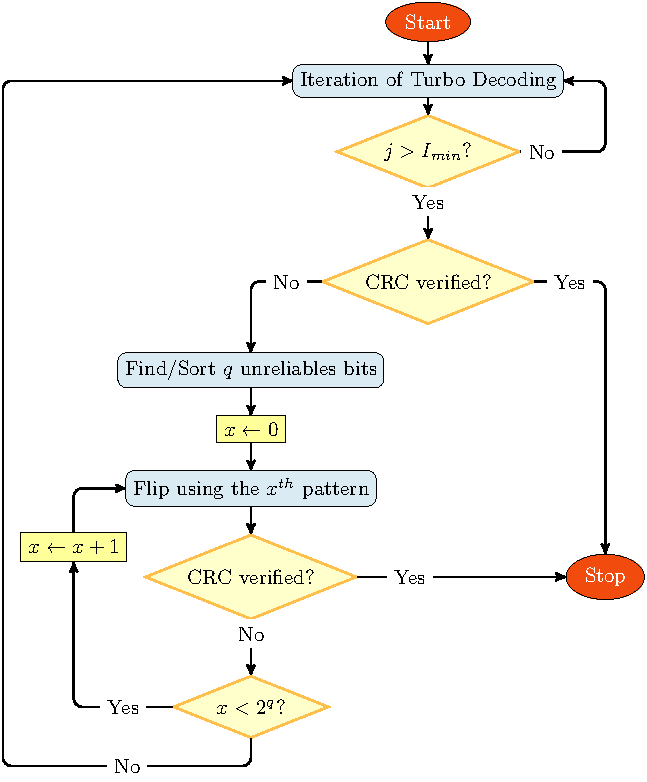
\includegraphics[width=\textwidth]{fig/flow/fc0.pdf}}
      % \only<2>{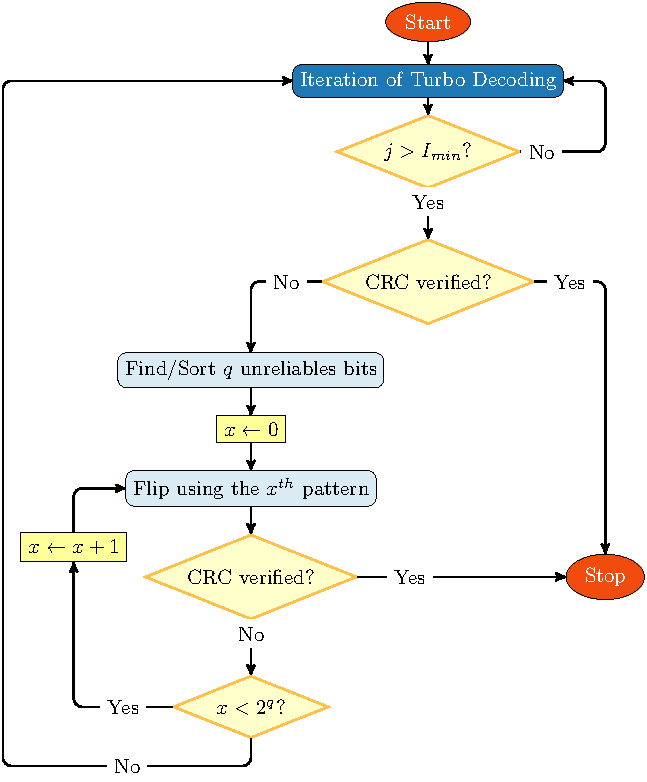
\includegraphics[width=\textwidth]{fig/flow/fc_tdec.pdf}}
      % \only<3>{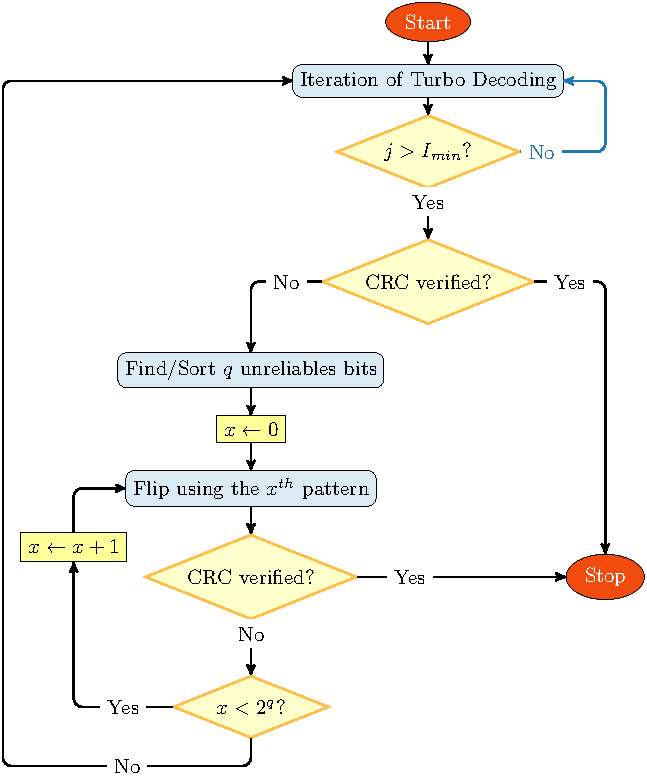
\includegraphics[width=\textwidth]{fig/flow/fc_reit.pdf}}
      % \only<4>{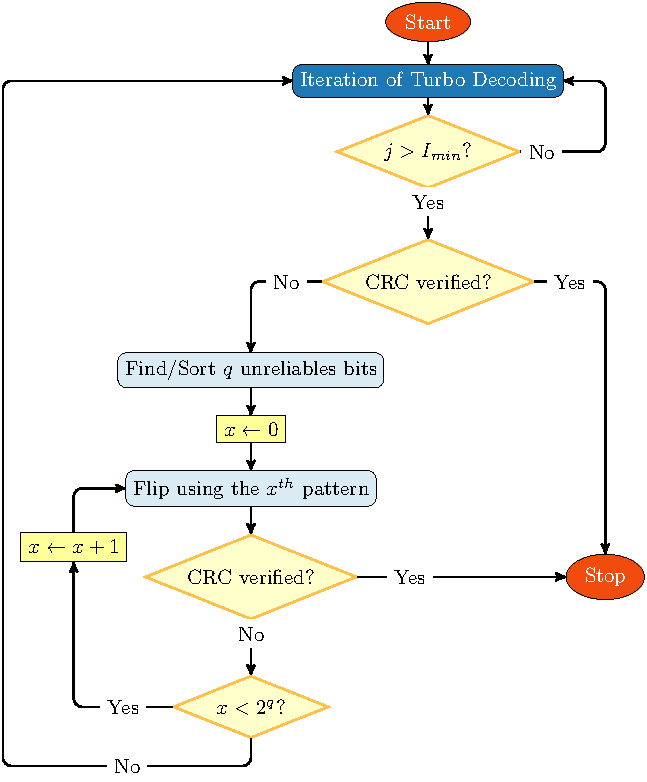
\includegraphics[width=\textwidth]{fig/flow/fc_tdec.pdf}}
      % \only<5>{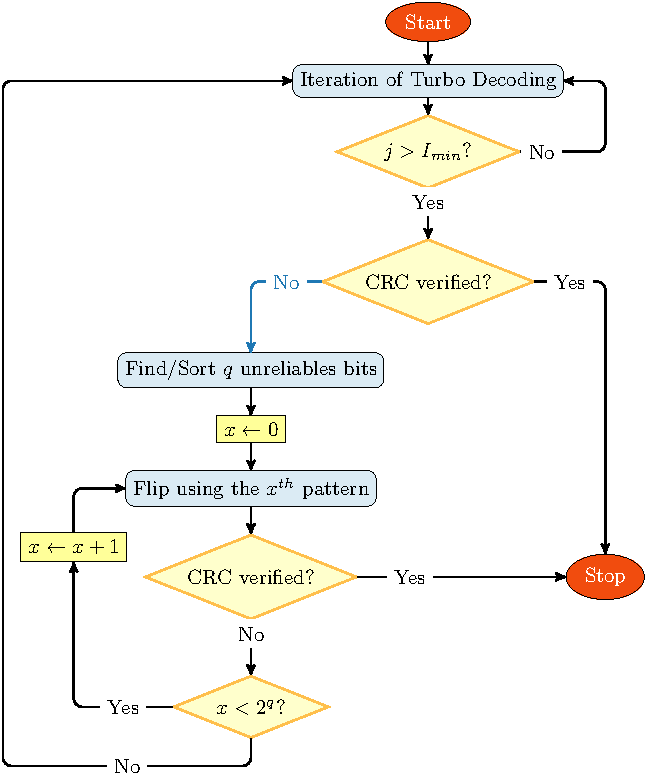
\includegraphics[width=\textwidth]{fig/flow/fc_nocrc.pdf}}
      % \only<6>{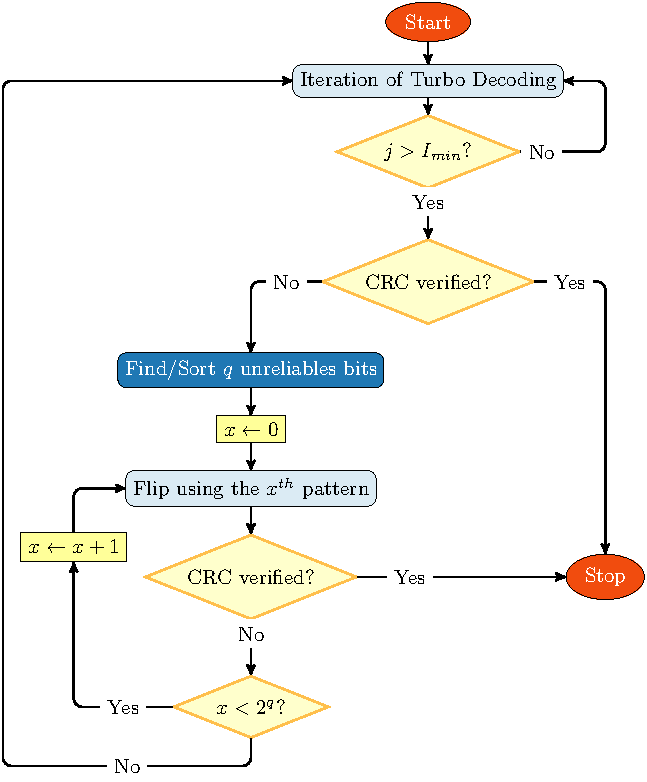
\includegraphics[width=\textwidth]{fig/flow/fc_find.pdf}}
      % \only<7>{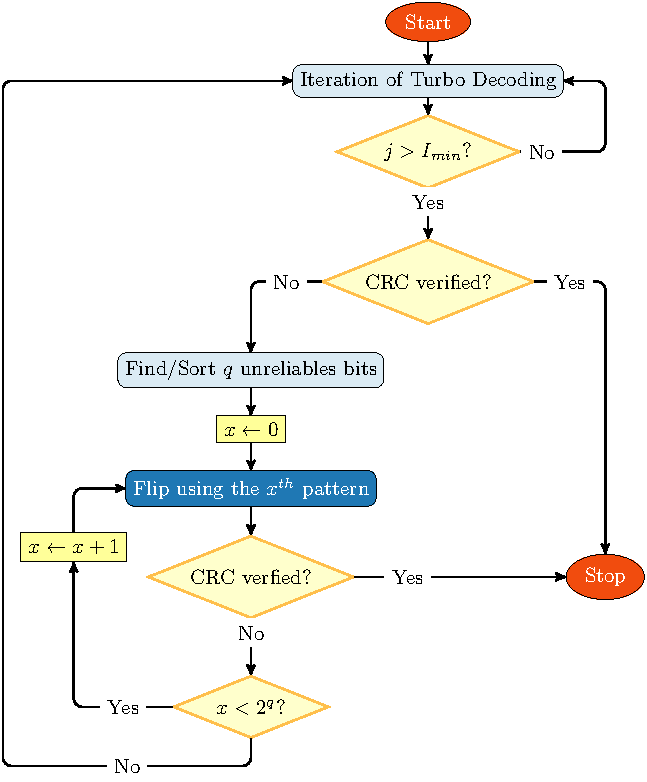
\includegraphics[width=\textwidth]{fig/flow/fc_flip.pdf}}
      % \only<8>{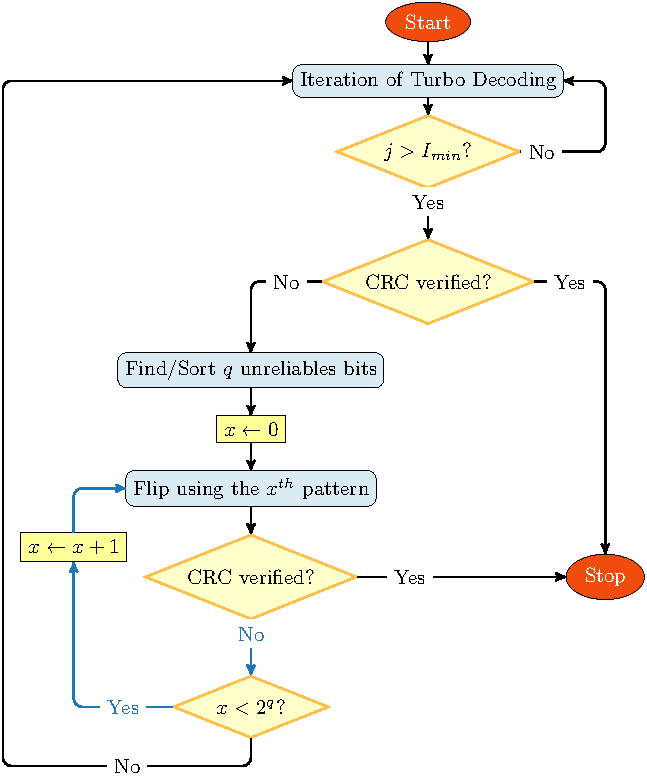
\includegraphics[width=\textwidth]{fig/flow/fc_flip2.pdf}}
      % \only<9>{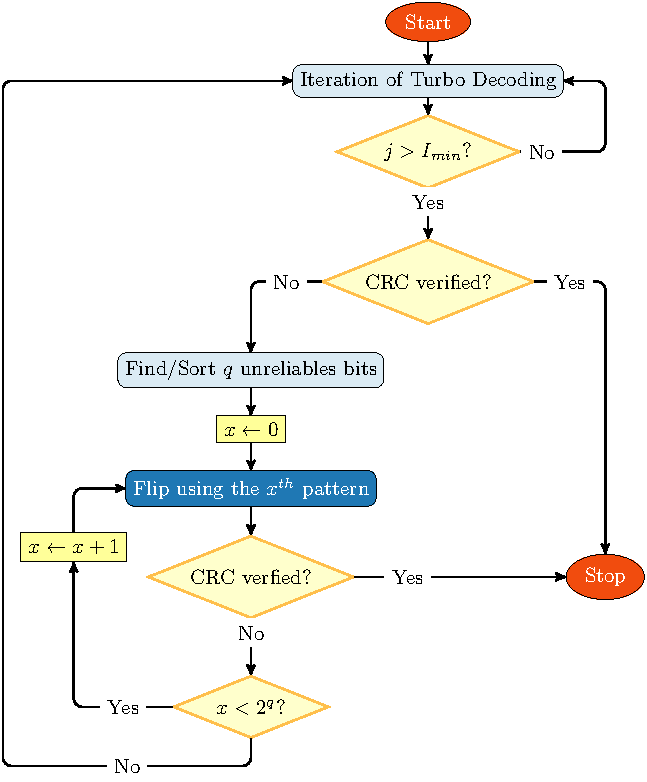
\includegraphics[width=\textwidth]{fig/flow/fc_flip.pdf}}
      % \only<10>{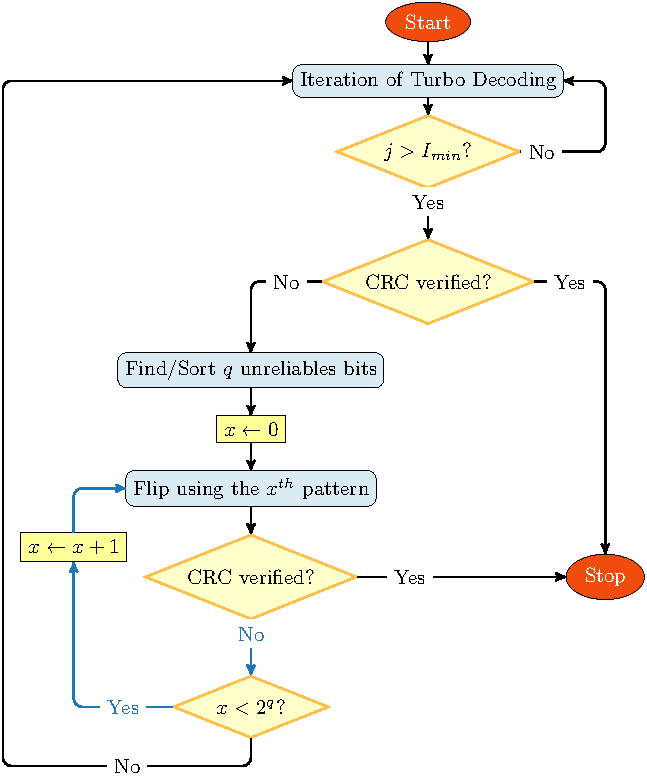
\includegraphics[width=\textwidth]{fig/flow/fc_flip2.pdf}}
      % \only<11>{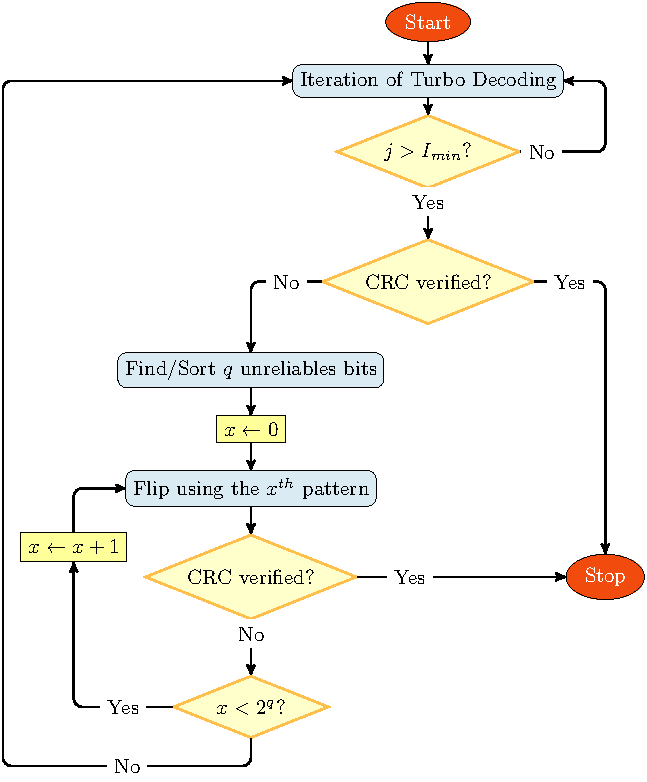
\includegraphics[width=\textwidth]{fig/flow/fc0.pdf}}
      \only<1>{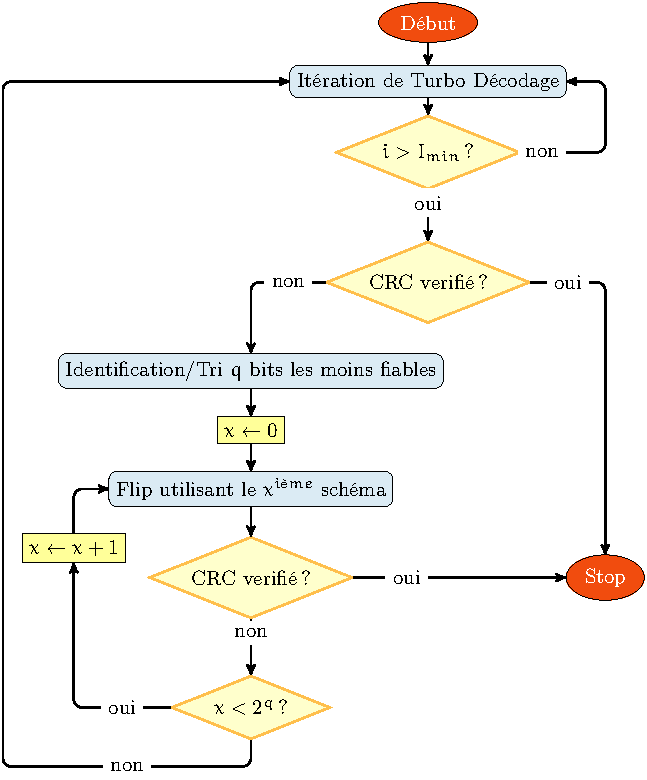
\includegraphics[width=\textwidth]{fig/flow/0.pdf}}
      \only<2>{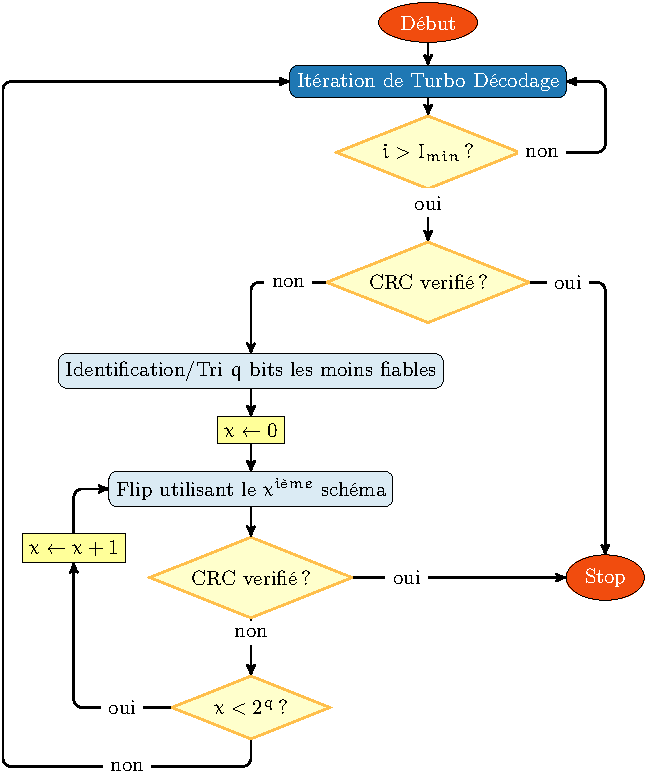
\includegraphics[width=\textwidth]{fig/flow/1.pdf}}
      \only<3>{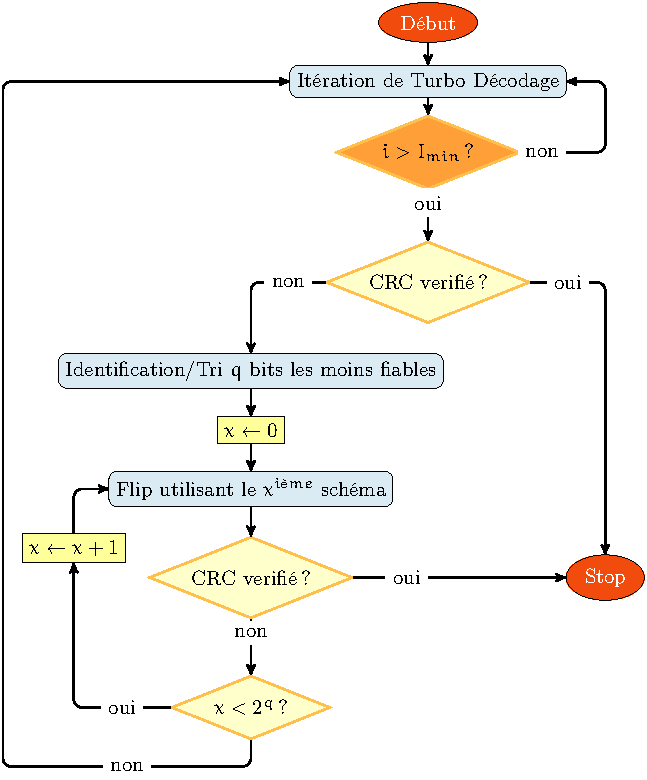
\includegraphics[width=\textwidth]{fig/flow/2.pdf}}
      \only<4>{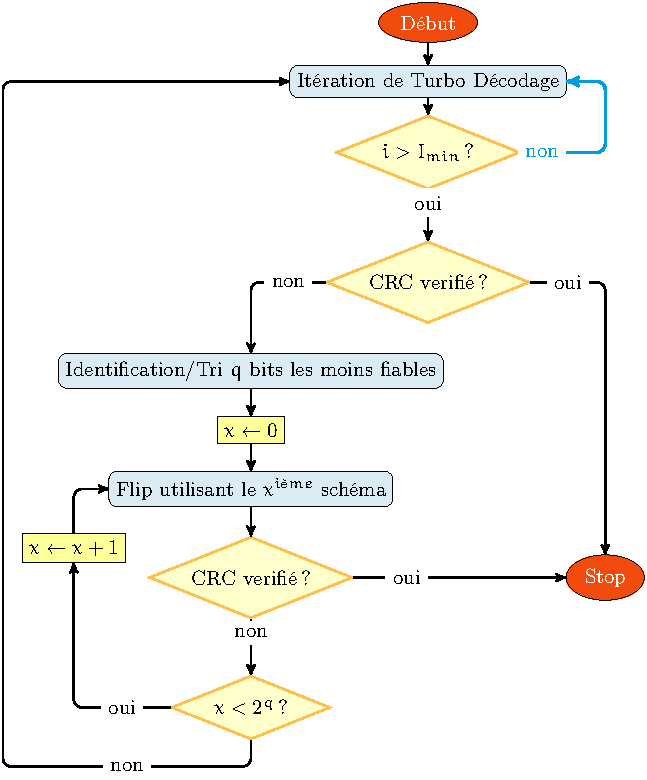
\includegraphics[width=\textwidth]{fig/flow/3.pdf}}
      \only<5>{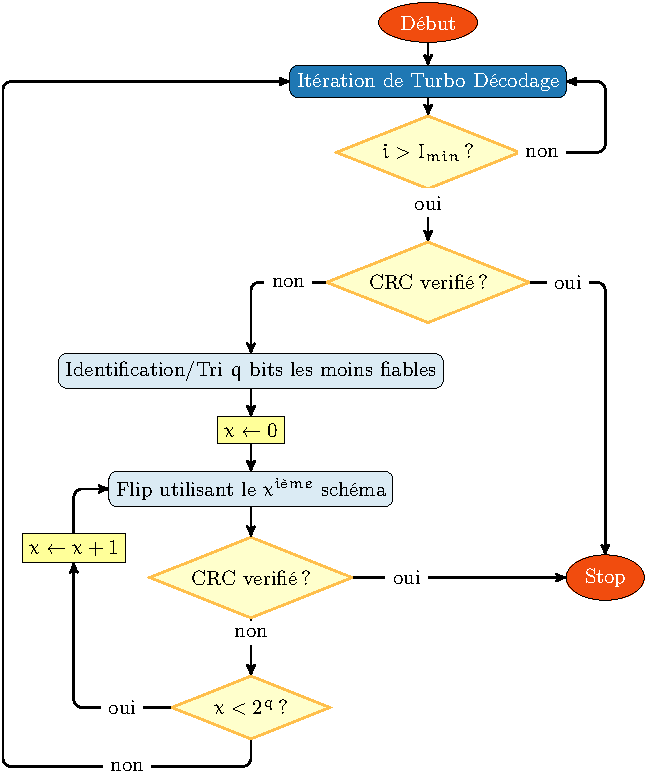
\includegraphics[width=\textwidth]{fig/flow/1.pdf}}
      \only<6>{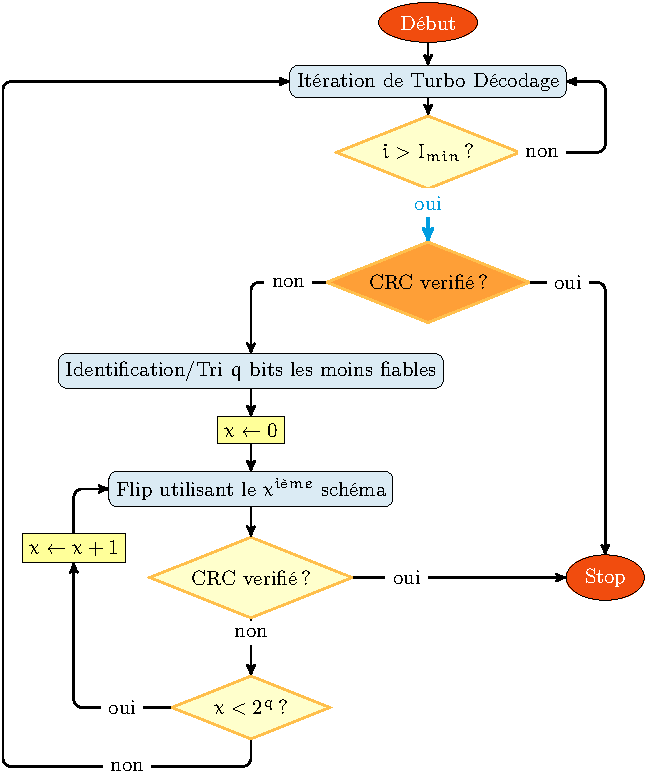
\includegraphics[width=\textwidth]{fig/flow/4.pdf}}
      \only<7-8>{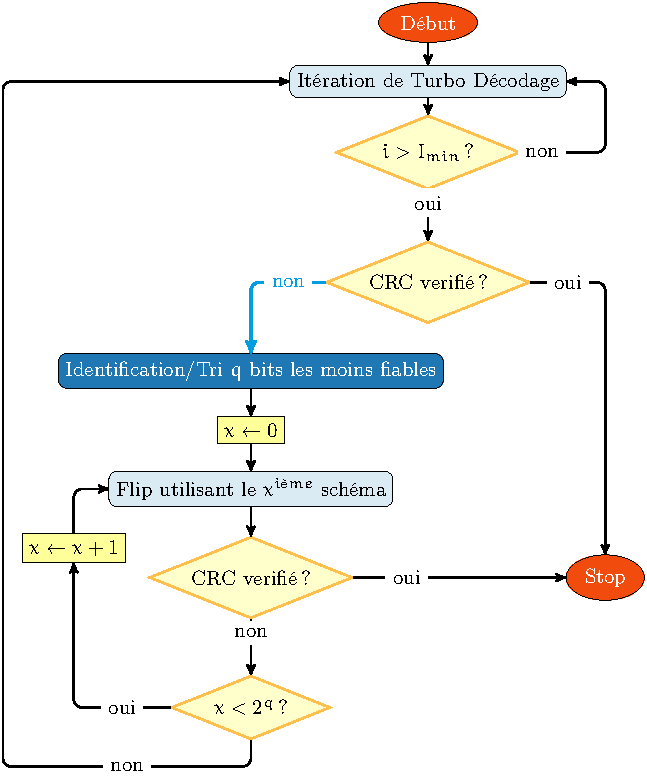
\includegraphics[width=\textwidth]{fig/flow/5.pdf}}
      \only<9-10>{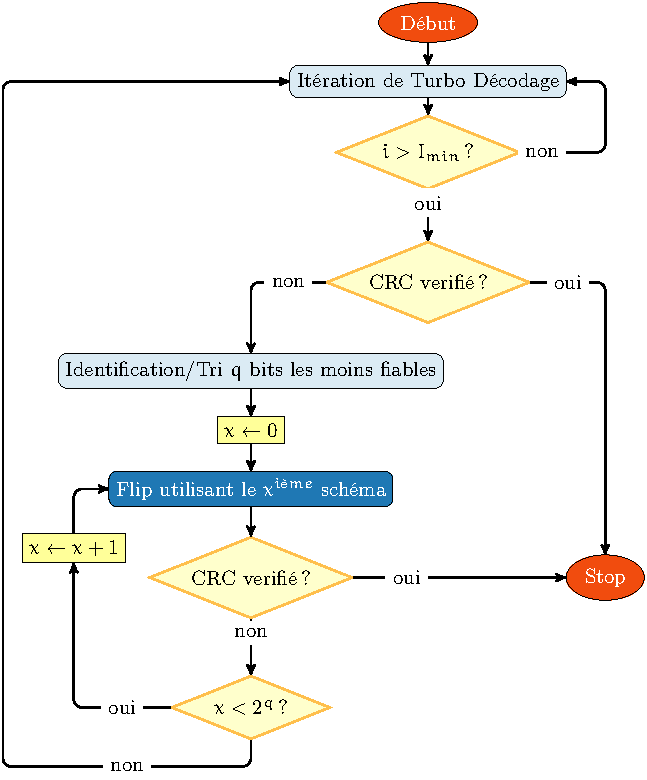
\includegraphics[width=\textwidth]{fig/flow/6.pdf}}
      \only<11>{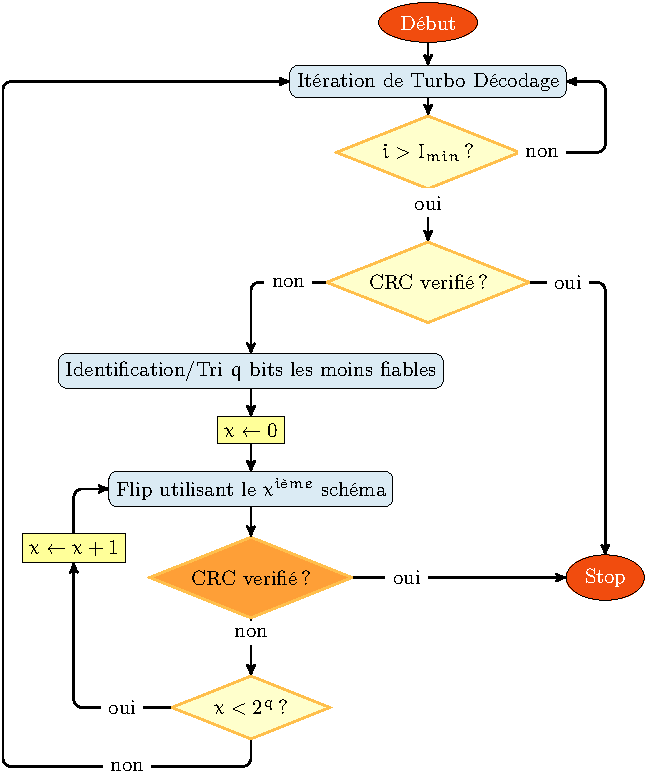
\includegraphics[width=\textwidth]{fig/flow/7.pdf}}
      \only<12>{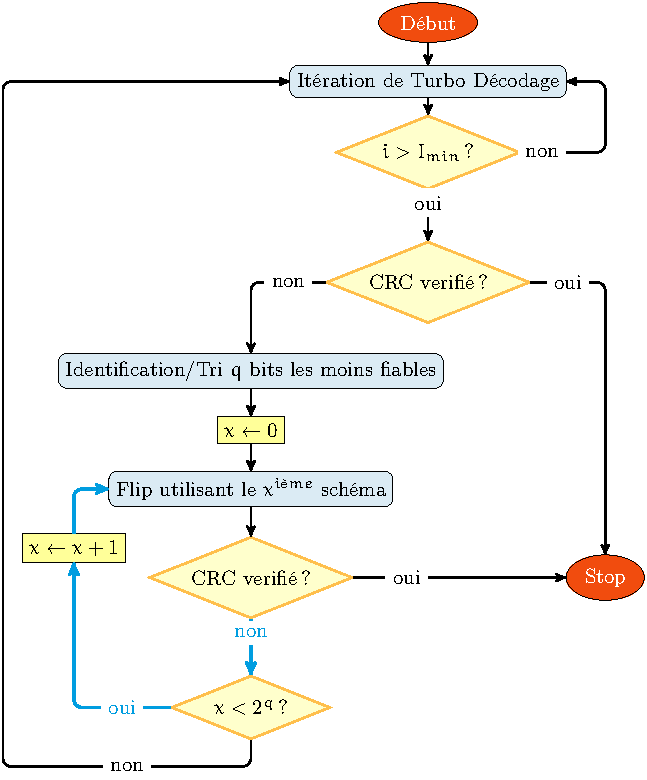
\includegraphics[width=\textwidth]{fig/flow/8.pdf}}
      \only<13>{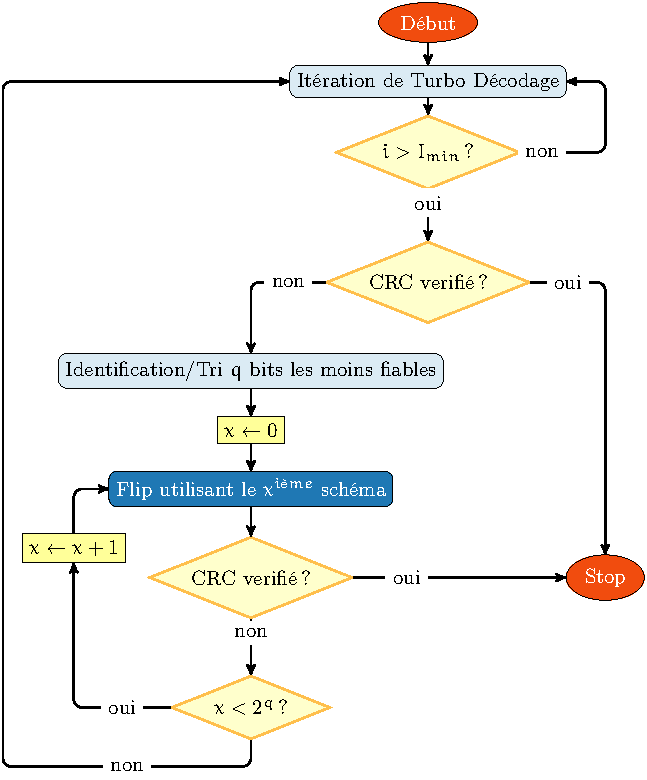
\includegraphics[width=\textwidth]{fig/flow/6.pdf}}
      \only<14>{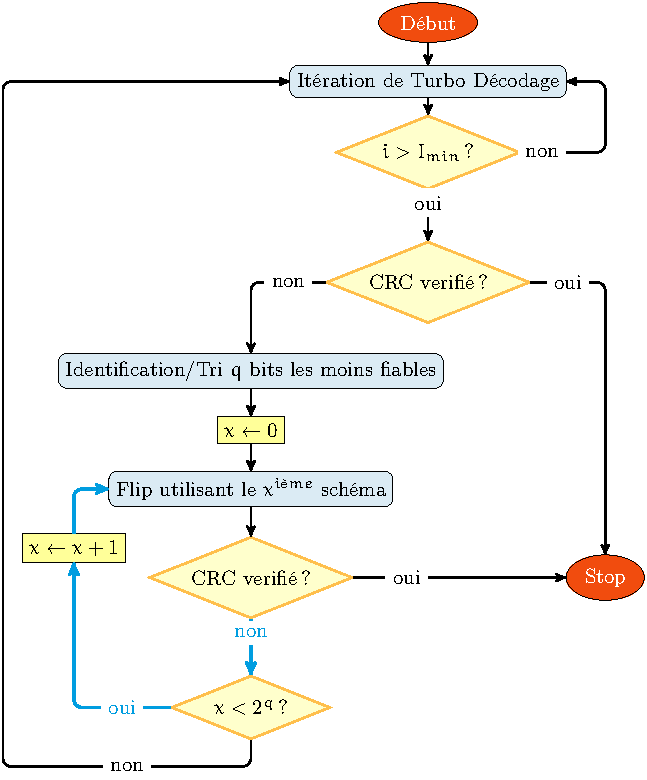
\includegraphics[width=\textwidth]{fig/flow/8.pdf}}
      \only<15-16>{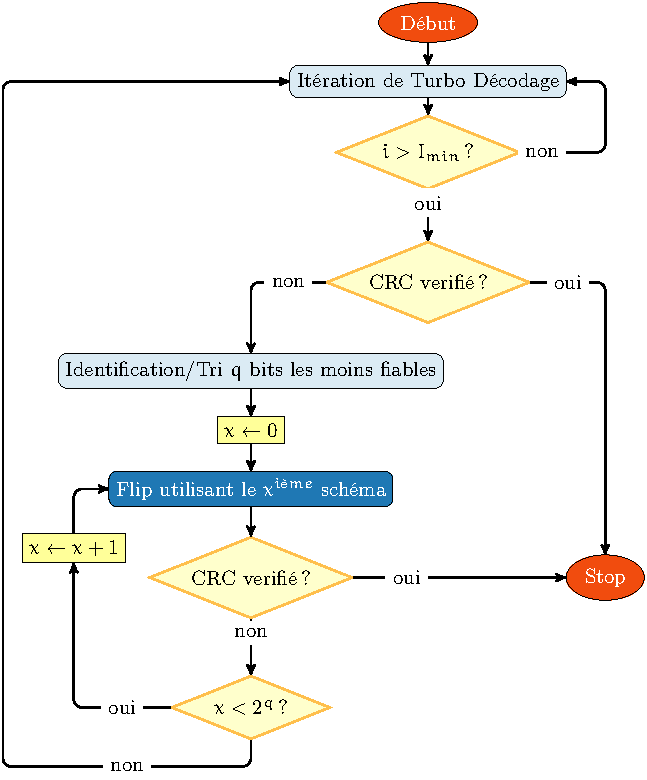
\includegraphics[width=\textwidth]{fig/flow/6.pdf}}
      \only<17>{\includegraphics[width=\textwidth]{fig/flow/10.pdf}}
      \only<18->{\includegraphics[width=\textwidth]{fig/flow/9.pdf}}
    \end{column}%
    \hfill%
    \begin{column}{.48\textwidth}
      \begin{center}
        \uncover<6->{
          \resizebox{\linewidth}{!}{
            \begin{tabular}{rllllllllll}
              & \multicolumn{7}{|c|}{\textit{bits d'information}} & \multicolumn{2}{|c|}{\textit{crc}} \\
              \toprule
              $\mathbf{\hat{d}}$ & \textcolor{Paired-5}{\textbf{0}}    & 1   & 1                                   & 0   & 1   & \textcolor{Paired-5}{\textbf{0}}    & 0   & 1   & 0   \\
              \uncover<7->{$\Delta$           & \only<8->{\cellcolor{Paired-6}}1.2 & 3.5 & \only<8->{\cellcolor{Paired-6}}0.2 & 4.2 & 5.1 & \only<8->{\cellcolor{Paired-6}}0.3 & 2.8 & 1.7 & 3.5 }\\
              \bottomrule
            \end{tabular}}  }
      \end{center}
      \only<8->{{\small$q = 3$ positions identifiées :}\resizebox{.31\linewidth}{!}{\begin{tabular}{ccc} 
        $k_2$ & $k_5$ & $k_0$ \\
        \end{tabular}}\\\vspace*{.2cm}}
      \only<9->{
        {\small$2^q - 1= 7$ mots candidats générés:}\\\vspace*{.2cm}
        \resizebox{\linewidth}{!}{\vspace*{.2cm}
          \begin{tabular}{rllllllllll}
            \toprule
            \only<9->{$\mathbf{d_1}$                                           & 0 ~~                                 & 1 ~~ & \only<10-16>{\cellcolor{Paired-4}}{0} ~~ & 0 ~~ & 1 ~~ & 0 ~~                                 & 0 ~~ & 1 ~~ & 0  }\\
            \only<13->{$\mathbf{d_2}$                                 & 0 ~~                                 & 1 ~~ & 1 ~~                                  & 0 ~~ & 1 ~~ & \only<13-16>{\cellcolor{Paired-4}}{1}   & 0 ~~ & 1 ~~ & 0} \\
            \only<15->{$\mathbf{d_3}$                                 & \only<13-16>{\cellcolor{Paired-4}}{1} ~~ & 1 ~~ & 1 ~~                                  & 0 ~~ & 1 ~~ & 0 ~~                                 & 0 ~~ & 1 ~~ & 0} \\
            \only<16->{$\mathbf{d_4}$                                & 0 ~~                                 & 1 ~~ & \only<13-16>{\cellcolor{Paired-4}}{0} ~~  & 0 ~~ & 1 ~~ & \only<13-16>{\cellcolor{Paired-4}}{1} ~~ & 0 ~~ & 1 ~~ & 0} \\
            \only<16->{$\mathbf{d_5}$                                & \only<13-16>{\cellcolor{Paired-4}}{1} ~~ & 1 ~~ & \only<13-16>{\cellcolor{Paired-4}}{0} ~~  & 0 ~~ & 1 ~~ & 0 ~~                                 & 0 ~~ & 1 ~~ & 0} \\
            \only<16->{\only<17>{\cellcolor{Paired-3}}$\mathbf{d_6}$ & \only<13-16>{\cellcolor{Paired-4}}{\textcolor{Paired-3}{\textbf{1}}} ~~ & 1 ~~ & 1 ~~                                  & 0 ~~ & 1 ~~ & \only<13-16>{\cellcolor{Paired-4}}{\textcolor{Paired-3}{\textbf{1}}} ~~ & 0 ~~ & 1 ~~ & 0} \\
            %\only<16->{$\mathbf{d_7}$                                & \only<13-16>{\cellcolor{Paired-4}}{1} ~~ & 1 ~~ & \only<13-16>{\cellcolor{Paired-4}}{0} ~~  & 0 ~~ & 1 ~~ & \only<13-16>{\cellcolor{Paired-4}}{1} ~~ & 0 ~~ & 1 ~~ & 0} \\
            \only<16->{$\mathbf{d_7}$                                &  &   &  &  &  &  &  & } \\
            \bottomrule
          \end{tabular}}\\\vspace*{.2cm}}
      %\only<17->{{\small} Ces mots sont vérifiés grace au CRC}
    \end{column}%
  \end{columns}
\end{frame}

\begin{frame}[c]{Performances de décodage - LTE, R=1/3, Canal AWGN, Flottant, 8 its}
\begin{center}
\begin{tikzpicture}
    \begin{semilogyaxis}[footnotesize, width=0.95\linewidth, height=0.6\linewidth,    
            xmin=0, xmax=3, xtick={0,0.5,...,3},
            %ymin=2e-6,  ymax=0.11,
            xlabel=$E_b/N_0 \text{(dB)}$, ylabel=FER,  grid=both, grid style={gray!30},
        tick align=outside, tickpos=left, %legend style={at={(0.5,-0.2)},anchor=north}]
        legend pos=north east]
        \addplot[mark=o,Paired-5, semithick, visible on=<2->]  table [x=SNR, y=FSF] {../main/ch3_fig/fnc/lte/dat/528};
        \addplot[mark=o,Paired-1, semithick, visible on=<4->]  table [x=SNR, y=FSF] {../main/ch3_fig/fnc/lte/dat/1024};
        \addplot[mark=o,Paired-3, semithick, visible on=<6->]  table [x=SNR, y=FSF] {../main/ch3_fig/fnc/lte/dat/2048};
        \addplot[mark=o,Paired-7, semithick, visible on=<6->]  table [x=SNR, y=FSF] {../main/ch3_fig/fnc/lte/dat/6144};
        \addplot[mark=o,Paired-5!50!Paired-6, semithick, dashed, mark options={solid}, visible on=<3->]  table [x=SNR, y=FER] {../main/ch3_fig/fnc/lte/dat/528};
        \addplot[mark=o,Paired-1!50!Paired-2, semithick, dashed, mark options={solid}, visible on=<5->]  table [x=SNR, y=FER] {../main/ch3_fig/fnc/lte/dat/1024};
        \addplot[mark=o,Paired-3!50!Paired-4, semithick, dashed, mark options={solid}, visible on=<6->]  table [x=SNR, y=FER] {../main/ch3_fig/fnc/lte/dat/2048};
        \addplot[mark=o,Paired-7!50!Paired-8, semithick, dashed, mark options={solid}, restrict x to domain=0.4:1.4, visible on=<6->]  table [x=SNR, y=FER] {../main/ch3_fig/fnc/lte/dat/6144};

        \legend{K=528, K=1024, K=2048, K=6144} 
         
    \end{semilogyaxis}
\end{tikzpicture}  
\end{center}
\end{frame}
%%%%%%%%%%%%%%%%%%%%%%%%%%%%%% ICI mon gros
\subsection[Double binaires]{Extension aux turbo codes doubles binaires}

\begin{frame}[c]{Introduction}
  \begin{block}{Les turbo codes double binaires}
  \begin{itemize}
  	\item Codage par symbole (couple de 2 bits)
  	\item Décodage par symbole
  \end{itemize}
 \end{block}
 \vspace*{3em}
 \begin{block}<2>{Extensions}
  \begin{itemize}
  	\item Métrique d'identification de symboles les moins fiables
  	\item Génération des mots candidats
  \end{itemize}
 \end{block}
\end{frame}

\begin{frame}[c]{Le critère pour les turbo codes double binaires}
  \begin{columns}[T] % align columns
    \begin{column}{.65\textwidth}
      \only<1>{\includegraphics[width=.9\textwidth, page=1, center]{fig/tdec_dbl.pdf}}
      \only<2->{\includegraphics[width=.9\textwidth, page=2, center]{fig/tdec_dbl.pdf}}
    \end{column}%
    \hfill%
    \begin{column}{.35\textwidth}
\only<3->{\begin{tabular}{@{}rllll@{}}
\toprule
$L_0$ & 1.2 \visible<5->{& 3.3 & 5.5 & 3.1} \\
$L_1$ & \only<4>{\textcolor{bleuUni}}{3.8} \visible<5->{& 3.5 & 1.3 & 4.4} \\
$L_2$ & 3.6 \visible<5->{& 0.2 & 1.1 & 4.0} \\
$L_3$ & \only<4>{\textcolor{bleuUni}}{5.5} \visible<5->{& 0.4 & 0.2 & 1.4} \\ 
\cmidrule(r){1-1} \cmidrule(l){2-5}
\only<4->{$\Delta$ & 1.7  \visible<5->{& 0.2 & 4.2 & 0.4}}\\ 
\bottomrule
\end{tabular}}
    \end{column}%
  \end{columns}
\visible<5->{\begin{itemize}\setlength\itemsep{2em}
  \item Considérer uniquement les deux symboles les plus probables : 
  \begin{equation*} \begin{split}
  {\quad \color{bleuUni}\bullet}\quad S_{M_x}(k) = \argmax\limits_{s\in\llbracket0;3\rrbracket}\left(L_s(k)\right)
  \end{split}\qquad
  \begin{split}
   {\color{bleuUni}\bullet}\quad S_{M_y}(k) = \argmax\limits_{s\in\llbracket0;3\rrbracket\setminus{S_{M_x}(k)}}\left(L_s(k)\right)
  \end{split} 
\end{equation*}
\begin{equation*}
  \Delta(k) = \mathbf{l^a_{S_{M_x}}(k)-l^a_{S_{M_y}}(k)}
\end{equation*}
\end{itemize}}
\end{frame}

\begin{frame}[c]{Génération des mots candidats}
\begin{itemize}\setlength\itemsep{2em}
  \item<1-> Considérer tous les symboles possibles par position est coûteux
  \item<2-> $4^q = 2^{2q}$ 
  \item<3-> D'après les études menées, majoritairement, si un symbole est erroné, alors le symbole émis correspond au deuxième plus probable ($S_{M_y}$)
\end{itemize}
\vspace*{1em}
\only<4->{{\color{bleuUni}\Large\MVRightarrow} Mémorisation des 2 symboles les plus probables et génération de $2^q$ mots candidats}
\end{frame}

\begin{frame}[c]{Algorithme FNC turbo codes double binaires}
% \begin{enumerate}\itmsp{1.5em}
%   \item Calcul de la métrique d'identification $\Delta$
%   \item Extraction des $q$ positions les moins fiables
%   \item Sauvegarde des deux symboles les plus probables à ces $q$ positions
%   \item Génération de $2^q - 1$ mots candidats
%   \item Vérification par le code CRC des mots candidats
% \end{enumerate}
\includegraphics[height=.9\textheight, center]{fig/flow/fc_dbl.pdf}
\end{frame}


% \begin{frame}[c]{Performances de décodage - DVB-RCS}
% \begin{center}
% \begin{tikzpicture}
%     \begin{semilogyaxis}[footnotesize, width=0.95\linewidth, height=0.6\linewidth,    
%             xmin=1, xmax=6, xtick={0,0.5,...,6},
%             %ymin=2e-6,  ymax=0.11,
%             xlabel=$E_b/N_0 \text{(dB)}$, ylabel=FER,  grid=both, grid style={gray!30},
%         tick align=outside, tickpos=left, %legend style={at={(0.5,-0.2)},anchor=north}]
%         legend pos=north east]
%         \addplot[mark=o,Dark2-1, semithick]  table [x=SNR, y=FER] {data/old/13}; 
%         \addplot[mark=diamond,Dark2-3, semithick]  table [x=SNR, y=FER] {data/old/12}; 
%         %\addplot[mark=triangle,Dark2-4, semithick]  table [x=SNR, y=FER] {data/old/23}; 
%         %\addplot[mark=square,Dark2-5, semithick]  table [x=SNR, y=FER] {data/old/34}; 
%         \addplot[mark=pentagon,Dark2-2, semithick]  table [x=SNR, y=FER] {data/old/45}; 
%         %\addplot[mark=oplus,Dark2-7, semithick]  table [x=SNR, y=FER] {data/old/67}; 
%     \end{semilogyaxis}
% \end{tikzpicture}  
% \end{center}
% \end{frame}

\begin{frame}[c]{Performances de décodage - {\footnotesize DVB-RCS2 - K=752 symb - QPSK - AWGN - 8 its - q=10}}
\begin{center}
\begin{tikzpicture}
    \begin{semilogyaxis}[footnotesize, width=0.95\linewidth, height=0.6\linewidth,    
            xmin=1, xmax=6, xtick={0,0.5,...,6},
            %ymin=2e-6,  ymax=0.11,
            xlabel=$E_b/N_0 \text{(dB)}$, ylabel=FER,  
            grid=both, grid style={gray!30},
          /pgfplots/table/ignore chars={|},
        tick align=outside, tickpos=left, %legend style={at={(0.5,-0.2)},anchor=north}]
        legend pos=north east]

        \addplot[mark=o,Paired-1, semithick, visible on =<2->]  table [x=Eb/N0, y=FER] {data/dvb2/dvb2_1504_12_ref.txt};
        \addplot[mark=o,Paired-3, semithick, visible on =<4->] coordinates { (3.6, 4.4e-5) (3.8, 3.7e-6) (4.0, 8.5e-7) (4.2, 2.6e-7) (4.4, 9.0e-8)};
        \addplot[mark=o,Paired-2!50!Paired-1, semithick, dashed, mark options={solid}, visible on =<3->]  table [x=Eb/N0, y=FER] {data/dvb2/dvb2_1504_12_fnc3.txt};
        \addplot[mark=o,Paired-4!50!Paired-3, semithick, dashed, mark options={solid}, visible on =<5->]  table [x=Eb/N0, y=FER] {data/dvb2/dvb2_1504_45_fnc3.txt};

        \legend{R=1/2, R=4/5}
    \end{semilogyaxis}
\end{tikzpicture}  
\end{center}
\end{frame}
%%%%%%%%%%%%%%%%%%%%%%%%%%%%%%%%%%%%%%%%%%%%%%%%%%%%%%%%%%%%%%%%%%%%%%%%%%%%%%%%
\section[Architecture matérielle]{Architecture matérielle de correction des erreurs résiduelles}
%%%%%%%%%%%%%%%%%%%%%%%%%%%%%%%%%%%%%%%%
\subsection{Les paramètres de l'algorithme FNC}
\begin{frame}[c]{Adéquation algorithme architecture}
\begin{itemize}\itmsp{2em}
  \item<1-> L'algorithme FNC est ajustable en fonction de plusieurs paramètres : 
    \begin{itemize}\itmsp{.5em}
    \item<2-> Nombre de mots candidats considérés\\\uncover<5->{{\color{bleuUni}\Large\MVRightarrow} Une position supplémentaire $\Rightarrow$ deux fois plus de vérifications de CRC}
    \item<3-> Itérations à l'issue desquelles le FNC est appliqué\\ \uncover<6-> {{\color{bleuUni}\Large\MVRightarrow} Modification du budget temps alloué}
  \end{itemize}
  \item<4-> Double impact : complexité calculatoire et performances de décodage
\end{itemize}
\end{frame}

% \begin{frame}[c]{Paramètres liés au processus itératif - Itération minimale}
% \begin{tikzpicture}
%   \begin{semilogyaxis}[footnotesize, width=0.95\linewidth, height=0.6\linewidth,
%   					xlabel=$E_b/N_0 \text{(dB)}$,   
%   					ylabel = FER, tick align=outside, tickpos=left,
% 					grid=both, grid style={gray!30},
% 					/pgfplots/table/ignore chars={|},
% 					xmin=0.4, xmax=1.8, xtick={0.4,0.6,...,1.8}, ymax=2,
% 					legend columns=2,
% 					%ymin= ,
% 					]
%         \addplot[mark=triangle,Set1-1, semithick, visible on=<2->]  table [x=Eb/N0, y=FER] {../main/ch4_fig/final/2048/ref.txt};
%         \addplot[mark=o,Set1-2, semithick, dashed, mark options={solid}, visible on=<3->]  table [x=Eb/N0, y=FER] {../main/ch4_fig/final/2048/fnc10_m2.txt};
%         \addplot[mark=o,Set1-3, semithick, dashed, mark options={solid}, visible on=<4->]  table [x=Eb/N0, y=FER] {../main/ch4_fig/final/2048/fnc10_m3.txt};
%         \addplot[mark=o,Set1-4, semithick, dashed, mark options={solid}, visible on=<5->]  table [x=Eb/N0, y=FER] {../main/ch4_fig/final/2048/fnc10_m4.txt};
%         \addplot[mark=o,Set1-5, semithick, dashed, mark options={solid}, visible on=<6->]  table [x=Eb/N0, y=FER] {../main/ch4_fig/final/2048/fnc10_m5.txt};
%         \addplot[mark=o,Set1-7, semithick, dashed, mark options={solid}, visible on=<7->]  table [x=Eb/N0, y=FER] {../main/ch4_fig/final/2048/fnc10_m6.txt};
%         \addplot[mark=o,Set1-8, semithick, dashed, mark options={solid}, visible on=<8->]  table [x=Eb/N0, y=FER] {../main/ch4_fig/final/2048/fnc10_m7.txt};
%         \addplot[mark=o,Set1-9, semithick, dashed, mark options={solid}, visible on=<9->]  table [x=Eb/N0, y=FER] {../main/ch4_fig/final/2048/fnc10_m8.txt}; 

%         \legend{TC conventionnel, FNC $I_\text{min}=2$, FNC $I_\text{min}=3$, FNC $I_\text{min}=4$, FNC $I_\text{min}=5$, 
%                 FNC $I_\text{min}=6$, FNC $I_\text{min}=7$, FNC $I_\text{min}=8$}
%     \end{semilogyaxis}
%     \end{tikzpicture}
% \end{frame}

% \begin{frame}[c]{Paramètres liés au processus itératif - Une seul itération}
% \begin{tikzpicture}
%   \begin{semilogyaxis}[footnotesize, width=0.95\linewidth, height=0.6\linewidth,
%   					xlabel=$E_b/N_0 \text{(dB)}$,   
%   					ylabel = FER, tick align=outside, tickpos=left,
% 					grid=both, grid style={gray!30},
% 					/pgfplots/table/ignore chars={|},
% 					xmin=0.4, xmax=1.8, xtick={0.4,0.6,...,1.8}, ymax=2,
% 					legend columns=2,
% 					%ymin= ,
% 					]
%      \addplot[mark=triangle,Set1-1, semithick, visible on=<2->]  table [x=Eb/N0, y=FER] {../main/ch4_fig/final/2048/ref.txt};
%         \addplot[mark=o,Set1-2, semithick, dashed, mark options={solid}, visible on=<3->]  table [x=Eb/N0, y=FER] {../main/ch4_fig/final/2048/fnc10_m5.txt};
%         \addplot[mark=o,Set1-3, semithick, dashed, mark options={solid}, visible on=<4->]  table [x=Eb/N0, y=FER] {../main/ch4_fig/final/2048/fnc10_m4_M4.txt};
%         \addplot[mark=o,Set1-4, semithick, dashed, mark options={solid}, visible on=<5->]  table [x=Eb/N0, y=FER] {../main/ch4_fig/final/2048/fnc10_m5_M5.txt};
%         \addplot[mark=o,Set1-5, semithick, dashed, mark options={solid}, visible on=<6->]  table [x=Eb/N0, y=FER] {../main/ch4_fig/final/2048/fnc10_m6_M6.txt};
%         \addplot[mark=o,Set1-7, semithick, dashed, mark options={solid}, visible on=<7->]  table [x=Eb/N0, y=FER] {../main/ch4_fig/final/2048/fnc10_m7_M7.txt};
%         \addplot[mark=o,Set1-8, semithick, dashed, mark options={solid}, visible on=<8->]  table [x=Eb/N0, y=FER] {../main/ch4_fig/final/2048/fnc10_m8.txt}; 

%         \legend{TC conventionnel, FNC $I_\text{min}=5$, FNC $@i=4$, FNC $@i=5$, FNC $@i=6$, FNC $@i=7$, FNC $@i=8$}
%     \end{semilogyaxis}
%     \end{tikzpicture}
% \end{frame}

% \begin{frame}[c]{Paramètres liés au processus itératif - Une seul itération}
% \begin{tikzpicture}
%   \begin{semilogyaxis}[footnotesize, width=0.95\linewidth, height=0.6\linewidth,
%   					xlabel=$E_b/N_0 \text{(dB)}$,   
%   					ylabel = FER, tick align=outside, tickpos=left,
% 					grid=both, grid style={gray!30},
% 					/pgfplots/table/ignore chars={|},
% 					xmin=0.4, xmax=1.8, xtick={0.4,0.6,...,1.8}, ymax=2,
% 					legend columns=2,
% 					%ymin= ,
% 					]
%     	  \addplot[mark=triangle,Set1-1, semithick, visible on=<2->]  table [x=Eb/N0, y=FER] {../main/ch4_fig/final/2048/ref.txt};
%         \addplot[mark=o,Set1-2, semithick, dashed, mark options={solid}, visible on=<3->]  table [x=Eb/N0, y=FER] {../main/ch4_fig/final/2048/fnc10_m5.txt};
%         \addplot[mark=o,Set1-3, semithick, dashed, mark options={solid}, visible on=<4->]  table [x=Eb/N0, y=FER] {../main/ch4_fig/final/2048/fnc10_m5_M8_s2.txt};

%         \legend{TC conventionnel, FNC $I_\text{min}=5$, FNC $@i=5 \text{et} 7$}
%     \end{semilogyaxis}
%     \end{tikzpicture}
% \end{frame}

\begin{frame}[c]{Variation du nombre de mots candidats - LTE, K=2048, R=1/3, 8its}
\begin{tikzpicture}
  \begin{semilogyaxis}[footnotesize, width=0.95\linewidth, height=0.6\linewidth,
            xlabel=$E_b/N_0 \text{(dB)}$,   
            ylabel = FER, tick align=outside, tickpos=left,
          grid=both, grid style={gray!30},
          /pgfplots/table/ignore chars={|},
          xmin=0.4, xmax=1.8, xtick={0.4,0.6,...,1.8}, ymax=2,
          legend columns=2,
          %ymin= ,
          ]

        \addplot[mark=triangle,Set1-1, semithick, visible on=<2->]  table [x=Eb/N0, y=FER] {../main/ch4_fig/final/2048/ref.txt};
        \addplot[mark=o,Set1-9, semithick, dashed, mark options={solid}, visible on=<3->]  table [x=Eb/N0, y=FER] {../main/ch4_fig/final/2048/fnc4_m5.txt};
        \addplot[mark=o,Set1-7, semithick, dashed, mark options={solid}, visible on=<4->]  table [x=Eb/N0, y=FER] {../main/ch4_fig/final/2048/fnc6_m5.txt};
        \addplot[mark=o,Set1-4, semithick, dashed, mark options={solid}, visible on=<5->]  table [x=Eb/N0, y=FER] {../main/ch4_fig/final/2048/fnc8_m5.txt};
        \addplot[mark=o,Set1-3, semithick, dashed, mark options={solid}, visible on=<6->]  table [x=Eb/N0, y=FER] {../main/ch4_fig/final/2048/fnc9_m5.txt};
        \addplot[mark=o,Set1-2, semithick, dashed, mark options={solid}, visible on=<7->]  table [x=Eb/N0, y=FER] {../main/ch4_fig/final/2048/fnc10_m5.txt};
       % \addplot[mark=o,Set1-5, semithick, dashed, mark options={solid}, visible on=<6->]  table [x=Eb/N0, y=FER] {../main/ch4_fig/final/2048/fnc7_m5.txt};
        %\addplot[mark=o,Set1-8, semithick, dashed, mark options={solid}, visible on=<8->]  table [x=Eb/N0, y=FER] {../main/ch4_fig/final/2048/fnc5_m5.txt};

      %\legend{TC conventionnel, FNC $q=10$, FNC $q=9$, FNC $q=8$, FNC $q=7$, FNC $q=6$, FNC $q=5$, FNC $q=4$}
      \legend{TC conventionnel, FNC $q=4$, FNC $q=6$, FNC $q=8$, FNC $q=9$, FNC $q=10$}
      \end{semilogyaxis}
    \end{tikzpicture}
\end{frame}

\begin{frame}[c]{Itérations à l'issue desquelles le processus FNC est appliqué - LTE, K=2048, R=1/3, 8its}
\begin{tikzpicture}
  \begin{semilogyaxis}[footnotesize, width=0.95\linewidth, height=0.6\linewidth,
            xlabel=$E_b/N_0 \text{(dB)}$,   
            ylabel = FER, tick align=outside, tickpos=left,
          grid=both, grid style={gray!30},
          /pgfplots/table/ignore chars={|},
          xmin=0.4, xmax=1.8, xtick={0.4,0.6,...,1.8}, ymax=2,
          legend columns=2,
          %ymin= ,
          ]
        \addplot[mark=triangle,Set1-1, semithick, visible on=<2->]  table [x=Eb/N0, y=FER] {../main/ch4_fig/final/2048/ref.txt};
        \addplot[mark=o,Set1-2, semithick, dashed, mark options={solid}, visible on=<3->]  table [x=Eb/N0, y=FER] {../main/ch4_fig/final/2048/fnc10_m2.txt};
        \addplot[mark=o,Set1-3, semithick, dashed, mark options={solid}, visible on=<4->]  table [x=Eb/N0, y=FER] {../main/ch4_fig/final/2048/fnc10_m5.txt};
        \addplot[mark=o,Set1-5, semithick, dashed, mark options={solid}, visible on=<5->]  table [x=Eb/N0, y=FER] {../main/ch4_fig/final/2048/fnc10_m5_M8_s2.txt};

        \legend{TC conventionnel \\ FNC $@i=2,3,4,5,6,7,8$ \\ FNC $@i=5,6,7,8$ \\ FNC $@i=5,7$ \\}
    \end{semilogyaxis}
    \end{tikzpicture}
\end{frame}


% \begin{frame}[c]{Quantification de la métrique $\Delta$}
% \begin{tikzpicture}
%   \begin{semilogyaxis}[footnotesize, width=0.95\linewidth, height=0.6\linewidth,
%   					xlabel=$E_b/N_0 \text{(dB)}$,   
%   					ylabel = FER, tick align=outside, tickpos=left,
% 					grid=both, grid style={gray!30},
% 					/pgfplots/table/ignore chars={|},
% 					xmin=0.2, xmax=1.5, xtick={0.2,0.7,...,1.5},
% 					%ymax=2,
% 					legend columns=2,
% 					%ymin= ,
% 					]

%         \addplot[mark=square, Set1-1, semithick, visible on=<2->]  table [x=Eb/N0, y=FER] {../main/ch4_fig/final/fp/6144_FP_8_bits_5.1_ref.txt};                       
%         \addplot[mark=square, Set1-2, semithick, dashed, mark options={solid}, visible on=<3->]  table [x=Eb/N0, y=FER] {../main/ch4_fig/final/fp/6144_FP_8_bits_5.1_FNC10.txt};    
%         \addplot[mark=square, Set1-3, semithick, dashed, mark options={solid}, visible on=<4->]  table [x=Eb/N0, y=FER] {../main/ch4_fig/final/8b/6144_FP_8_bits_5.1_FNC10_7b.txt};    
%         \addplot[mark=square, Set1-4, semithick, dashed, mark options={solid}, visible on=<5->]  table [x=Eb/N0, y=FER] {../main/ch4_fig/final/8b/6144_FP_8_bits_5.1_FNC10_6b.txt};    
%         \addplot[mark=square, Set1-5, semithick, dashed, mark options={solid}, visible on=<6->]  table [x=Eb/N0, y=FER] {../main/ch4_fig/final/8b/6144_FP_8_bits_5.1_FNC10_5b.txt};    
%         \addplot[mark=square, Set1-7, semithick, dashed, mark options={solid}, visible on=<7->]  table [x=Eb/N0, y=FER] {../main/ch4_fig/final/8b/6144_FP_8_bits_5.1_FNC10_4b.txt};    
%         \addplot[mark=square, Set1-8, semithick, dashed, mark options={solid}, visible on=<8->]  table [x=Eb/N0, y=FER] {../main/ch4_fig/final/8b/6144_FP_8_bits_5.1_FNC10_4b_div2.txt};    
			
% 			\legend{TC conventionnel, FNC $b_\Delta=8$, FNC $b_\Delta=7$, FNC $b_\Delta=6$, FNC $b_\Delta=5$, FNC $b_\Delta=4$, FNC $b_\Delta=8$ div2}
%     \end{semilogyaxis}
%     \end{tikzpicture}
% \end{frame}


\begin{frame}[c]{Conclusion sur l'impact des paramètres de l'algorithme}
\begin{enumerate}\itmsp{2em}
  \item<1-> Nombre de mots candidats :
  \begin{itemize}
    \item<1-> Augmenter le nombre de mots candidats augmente le pouvoir de correction
    \item<1-> Mais la complexité calculatoire est aussi augmentée
	\end{itemize}
    \item<2-> Itérations :
  \begin{itemize}
    \item<2-> Appliquer trop tôt le FNC est problématique : faux positifs du CRC
    \item<2-> Cela dépend du pouvoir de détection du CRC et donc de la taille de la trame
    \item<2-> Il est possible de réduire le nombre d'applications tout en conservant les gains
	\end{itemize}
\end{enumerate}
\vspace*{2em}
\only<3->{{\color{bleuUni}\Large\MVRightarrow} Choix des paramètres à définir par le concepteur suivant le compromis entre les gains de décodage et le surcoût matériel acceptable}
\end{frame}
%%%%%%%%%%%%%%%%%%%%%%%%%%%%%%%%%%%%%%%%
% \subsection{Implantation matérielle de turbo décodeurs}
% \begin{frame}[c]{les ordonancement de turbo décodeurs}
%     \begin{itemize}
%     	\item Il existe une grande variété d'architectures et d'ordonnancements de turbo décodeurs
%     	\item Adressent des objectifs de débit et de complexité matérielle variés
%     	\item FNC : \og verrue \fg connectée à un turbo décodeur
%     \end{itemize}
% \vspace*{2em}
% \begin{center}
% \begin{tabular}{rll}
% \toprule
% Ordonnancement     & \begin{tabular}[c]{@{}l@{}}Durée d'une \\ demi-itération\end{tabular} & \begin{tabular}[c]{@{}l@{}}Nombre d'informations \\\textit{a posteriori} simultanées\end{tabular}     \\
% \cmidrule(r){1-1}  \cmidrule(l){2-2}        \cmidrule(l){3-3} 
% \uncover<2->{FB 		             & $2\times K$          & 1            }\\
% \uncover<3->{BF-SW (W)          & $K + \ddfrac{K}{W}$  & 1            }\\
% \uncover<4->{BFLY               & $K$                  & 2            }\\
% \uncover<5->{BFLY-SW (W)        & $K$                  & 2            }\\
% \uncover<6->{BFLY-SB (B)        & $\ddfrac{K}{B}$      & $2\times B$  }\\
% \uncover<7->{BFLY-SW-SB (W,B)   & $\ddfrac{K}{B}$      & $2\times B$  }\\
% \bottomrule
% \end{tabular}
% \end{center}
% \end{frame}

% \begin{frame}[c]{Ordonnancement retenu}
% \includegraphics[width=.8\columnwidth, right]{../main/ch4_fig/ipe/BF_SW+LEG.pdf}
%   \captionof{figure}{Ordonnancement BCJR Retour-Aller avec fenêtre glissante, W=2 (BF-SW).}
% \vspace*{2ex}
%   \resizebox{1\textwidth}{!}{
% \begin{tabular}{rllll}
% \toprule
% Ordonnancement      & \begin{tabular}[c]{@{}l@{}}Durée d'une \\ demi-itération\end{tabular} & \begin{tabular}[c]{@{}l@{}}Durée d'une \\ itération\end{tabular} & \begin{tabular}[c]{@{}l@{}}Durée de la transmission \\ d'informations \textit{a posteriori} \end{tabular} & \begin{tabular}[c]{@{}l@{}}Nombre d'informations \\\textit{a posteriori} simultanées\end{tabular}     \\
% \cmidrule(r){1-1}   \cmidrule(l){2-2}        \cmidrule(l){3-3} \cmidrule(l){4-4}                  \cmidrule(l){5-5}    
% BF-SW (W)           & $K + \ddfrac{K}{W}$  & $2\times(K + \ddfrac{K}{W})$ & $K$                    & 1               \\
% \bottomrule
% \end{tabular}}
% \end{frame}


%%%%%%%%%%%%%%%%%%%%%%%%%%%%%%%%%%%%%%%%
\subsection{Implantation matérielle de l'algorithme FNC}
% \begin{frame}[c]{Principe et ordonnancement}
%   \includegraphics{../main/ch4_fig/ipe/fnc_tc.pdf}
% \end{frame}

\begin{frame}[c]{Interconnexion entre le turbo décodeur et l'architecture FNC}
    \includegraphics[width=.9\textwidth, page=1, center]<1>{fig/serial.pdf}
    \includegraphics[width=.9\textwidth, page=2, center]<2>{fig/serial.pdf}
    \includegraphics[width=.9\textwidth, page=3, center]<3>{fig/serial.pdf}
    \includegraphics[width=.9\textwidth, page=4, center]<4>{fig/serial.pdf}
\end{frame}

\begin{frame}[c]{Ordonnancement du système [ turbo décodeur + module FNC ]}
    \includegraphics[height=.94\textheight, page=1, center]<1>{fig/fnc_tc.pdf}
    \includegraphics[height=.94\textheight, page=2, center]<2>{fig/fnc_tc.pdf}
    % \includegraphics[height=.94\textheight, page=3, center]<3>{fig/fnc_tc.pdf}
    % \includegraphics[height=.94\textheight, page=4, center]<4>{fig/fnc_tc.pdf}
    \includegraphics[height=.94\textheight, page=5, center]<3>{fig/fnc_tc.pdf}
\end{frame}

\begin{frame}[c, fragile]{Architecture du module FNC : Vue d'ensemble et détails}
    \includegraphics[width=.9\textwidth, page=1, center]<1>{fig/fnc_arch.pdf}
    \includegraphics[width=.9\textwidth, page=2, center]<2>{fig/fnc_arch.pdf}
    \includegraphics[width=.9\textwidth, page=3, center]<3>{fig/fnc_arch.pdf}
    \includegraphics[width=.9\textwidth, page=4, center]<4>{fig/fnc_arch.pdf}
    \includegraphics[width=.9\textwidth, page=5, center]<5>{fig/fnc_arch.pdf}
    \includegraphics[width=.9\textwidth, page=6, center]<6>{fig/fnc_arch.pdf}
  \end{frame}  
    
\begin{frame}[c]{Résultats d'implantation - Paramètres}
\begin{columns}[T]
\begin{column}{.5\textwidth}
\vspace*{2em}
  \begin{itemize}\setlength{\itemsep}{1.5em}
    \item Architecture décrite en VHDL {\color{bleuUni}\Large\MVRightarrow} FPGA
    \item Description générique avec $K$ et $q$
    \item K=6144, pire cas {\color{bleuUni}\Large\MVRightarrow} 1 bloc RAM utilisé (Xilinx, 18 Kbits). 
  \end{itemize}
  \end{column}%
  \hfill%
  \begin{column}{.5\textwidth}
  	\includegraphics[width=\textwidth]{fig/nexys.jpg}
  \end{column}
  \end{columns}
\end{frame}
    
    
% \begin{frame}[c]{Résultats d'implantation - Comparaison avec IP turbo decoder}
%   \begin{center}
%     \begin{table}[!t]
%       \caption{FPGA synthesis results for turbo decoder architecture (Xilinx IP)}
%       \label{tab:fpga_soa}
%       \begin{tabular}{lrrrrrrr} 
%         \toprule
%         LUT  & FF   & Slices & BRAM & f (MHz) & T/P (Mbps)      & WER @ 1 dB         \\ 
%         \midrule
%         3712 & 4062 & 3765   & 13   & 285     & $\sim$ 17 ($I_{TC} = 8$) & 1.7e-5\\ 
%         \bottomrule 
%       \end{tabular}
%     \end{table}
                                                                                                                                                                                                                                                                                                                                                                                        
%     \begin{table}[!t]
%       \centering
%       \caption{FPGA synthesis results for the FC algorithm }
%       \label{tab:fpga_fc_v7}
%       \only<1>{   \begin{tabular}{lrrrrrr} 
%         \toprule
%         $\mathbf{q}$ & LUT & FF & Paired & BRAM & f (MHz)& WER @ 1 dB\\ 
%         \midrule 
%         \textbf{4} & 595 & 572 & 670 & 1 & 224 & 3e-6\\ 
%         \textbf{6} & 1620 & 1952 & 1955 & 1 & 208 & 1.1e-6\\ 
%         \textbf{8} & 5376 & 7052 & 6542 & 1 & 129 & 8e-7\\ 
%         \textbf{10} & 15402 & 24883 & 23472 & 1 & 93 & 6e-7\\ 
%         \bottomrule 
%         \end{tabular} }
%     \end{table}
%   \end{center}
% \end{frame}
\begin{frame}{Résultats d'implantation - Circuit FPGA \bsc{Xilinx Virtex-6} \bsc{xc6vlx75t-1}}
	\begin{center}
	\only<1>{\vspace*{-1.5em}}
	\only<2->{\vspace*{-1em}}
	\resizebox*{.6\textwidth}{!}{
	\begin{tabular}{lrrrrr} 
		\toprule
		$q$ & LUT   & FF    & Slices & BRAM & f (MHz) \\ 	\cmidrule(r){1-1}\cmidrule(l){2-6}
		4   &  533  &  539  & 610    & 1	  & 293     \\
		6   & 1438  & 1725  & 1844   & 1    & 216     \\
		8   & 4283  & 6267  & 5731   & 1    & 172     \\
		10  & 15193 & 24833 & 23720  & 1    & 103     \\
		\bottomrule \vspace*{-.5em}
	\end{tabular}}
	\end{center}
	\only<2-5>{\begin{columns}[T]
	\begin{column}{.6\textwidth}
	\includegraphics[width=.9\textwidth]<2-5>{../main/ch4_fig/implem/xc6_4.pdf}
	  \end{column}%
  \hfill%
  \begin{column}{.5\textwidth}
	\includegraphics[width=.8\textwidth]<3>{chart/chart_4.pdf}
	\includegraphics[width=.8\textwidth]<4>{chart/chart_6.pdf}
	\includegraphics[width=.8\textwidth]<5>{chart/chart_10.pdf}
	  \end{column}
  \end{columns}}
  	\only<6->{%
  	\begin{columns}[T]
			\begin{column}{.6\textwidth}
			\vspace{1em}
			\centering
			IP Core Xilinx :\\
			\vspace{.5em}
			\resizebox*{\textwidth}{!}{%
  			\begin{tabular}{lrrrrrr} 
					\toprule
					LUT & FF & Slices & BRAM & f (MHz)& T/P (Mbps) \\ 
					\midrule
					3712 & 4062 & 3765 & 13 & 285 & $\sim$ 17 ($I_{TC} = 8$)\\ 
					\bottomrule 							\vspace{2em}
				\end{tabular}}

							\resizebox*{.6\textwidth}{!}{%
  			\begin{tabular}{lrr} 
					\toprule
					 & FER @ 1 dB & Slices (ratio)\\ 
					\cmidrule(r){2-2} \cmidrule(r){3-3}
					\uncover<7->{TC & $1,5\times10^{-5}$ & }\\
					\uncover<8->{$q=4$ & $3\times10^{-6}$ & $16\%$}\\
					\uncover<9->{$q=6$ & $1,2\times10^{-6}$ & $49\%$}\\
					\uncover<10->{$q=10$ & $7,2\times10^{-7}$ & $630\%$}\\
					\bottomrule 
				\end{tabular}}
			\end{column}%
  		\hfill%
  		\begin{column}{.4\textwidth}
  		\begin{tikzpicture}
 				\begin{semilogyaxis}[footnotesize, width=\linewidth, height=1.18\linewidth,    
      		xmin=0.7, xmax=1.2, xtick={0.7,0.8,...,1.2},
      		ymin=8e-8,  ymax=5E-3,
      xlabel=$E_b/N_0~\text{(dB)}$, 
      %ylabel=\only<1>{Taux d'erreur binaire}\only<2->{Probabilité et taux d'erreurs binaires},
      ylabel=FER,
      grid=both, grid style={gray!30},
      tick align=outside, tickpos=left, % legend columns=2, legend style={at={(1, -.25), anchor=north}, /tikz/column 2/.style={column sep=5pt}} 
      ]

			\addplot[mark=diamond,Paired-5, mark options=solid, visible on=<7->]  table [x=SNR, y=q0] {data/6144_qvar}; 
			\addplot[mark=diamond,Paired-3,dashed, mark options=solid, visible on=<8->]  table [x=SNR, y=q4] {data/6144_qvar}; 
			\addplot[mark=diamond,Paired-7,dashed, mark options=solid, visible on=<9->]  table [x=SNR, y=q6] {data/6144_qvar}; 
			\addplot[mark=diamond,Paired-1,dashed, mark options=solid, visible on=<10->]  table [x=SNR, y=q10] {data/6144_qvar};

	      \legend{TC, q=4, q=6, q=10}                                                                                               
  \end{semilogyaxis}
\end{tikzpicture}
  		\end{column}
  	\end{columns}}
\end{frame} 

%%%%%%%%%%%%%%%%%%%%%%%%%%%%%%%%%%%%%%%%%%%%%%%%%%%%%%%%%%%%%%%%%%%%%%%%%%%%%%%%
\section[Conclusion]{Conclusion et perspectives}

\begin{frame}[fragile]{Conclusion}
% \begin{enumerate}\itmsp{1em}
%   \item<1-> Propositions d'algorithmes améliorant les performance de décodage des turbo codes
%   \begin{itemize}
%     \item<2-> Self-Corrected : Sous certaines conditions, gain d'un ordre de grandeur dans la convergence\\
%     \only<3->{\color{marronUni} “L’algorithme Self-Corrected Max-Log-MAP pour le décodage des turbo codes” - JNRDM - 2015\\
%     “Extension du principe self-corrected de l’information extrinsèque au décodage itératif de turbo codes” - GRETSI - 2015}
%     \item <4-> Algorithme Flip And Check : Gain d'environ un ordre de grandeur dans la zone du plancher d'erreurs\\
%      \only<5->{\color{marronUni} “Lowering the error floor of turbo codes with CRC verifications” - IEEE Wireless Commun. Lett. - 2016\\
%      “Lowering the error floor of double-binary turbo codes : The flip and check algorithm,” - ISTC - 2016}
%   \end{itemize}
%   \item<6-> Architecture matérielle pour l'algorithme FNC\\
%   \only<7->{\small \color{marronUni} “Hardware architecture for lowering the error floor of lte turbo codes” - DASIP - 2016\\
%   “Correction des erreurs résiduelles lors du processus de turbo décodage :
% algorithme et architecture” - GDR Soc-SiP - 2017}
% \end{enumerate}

\begin{enumerate}\itmsp{1em}
  \item<1-> Propositions d'algorithmes améliorant les performance de décodage des turbo codes
  \begin{itemize}\itmsp{.5em}
    \item<2-> Self-Corrected : Sous certaines conditions, gain d'un ordre de grandeur dans la convergence\\
    \only<3->{\color{bleuUni} [JNRDM 2015]\\} 
    \only<3->{\color{bleuUni} [GRETSI 2015]}
    \item <4-> Algorithme Flip And Check : Gain d'environ un ordre de grandeur dans la zone du plancher d'erreurs\\
     \only<5->{\color{bleuUni} [IEEE Wireless Commun. Lett.  2016]\\}
     \only<5->{\color{bleuUni} [ISTC 2016]}
  \end{itemize}
  \item<6-> Architecture matérielle pour l'algorithme FNC\\
  \only<7->{\color{bleuUni} [DASIP 2016]\\}
  \only<7->{\color{bleuUni} [GDR SoC-SiP 2017]}
\end{enumerate}
\end{frame}

\begin{frame}[c]{Perspectives}
\begin{enumerate}\itmsp{2em}
  \item<1-> Algorithmiques
  \begin{itemize}
    \item<2-> Adaptation pour les codes LDPC
    \item<2-> Ordonner la génération des mots candidats de façon plus optimisée
  \end{itemize}
  \item<1-> Architecturales
    \begin{itemize}
    \item<3-> Réduire la complexité
    \item<3-> Compatibilité avec autres ordonnancements de turbo codes binaires
    \item<3-> Support des turbo codes doubles binaires
  \end{itemize}
  \item<1-> Industrielle
  \begin{itemize}
    \item<4-> Exploiter un modèle de canal aéronautique
  \end{itemize}
\end{enumerate}
\end{frame}

\begin{frame}[c]{Merci}
\begin{center}
Merci pour votre attention !
\end{center}
\end{frame}

\end{document}



